%!TEX root = Manuscrit.tex
\chapter{Cartographie automatisée d'images aériennes}
	\citationChap{}{}
	\minitoc
	\newpage

%%%%%%%%%%%%%%%%%%%%%%%%%%%%%%%%%%%%%%%%%%%%%%%%%%%%%%%%%%%%%%%%%%%%%%%%%%%%%%%%%%%%%%%%%%%%%

\section{Méthodes de cartographie d'images de télédétection}

\begin{figure}
	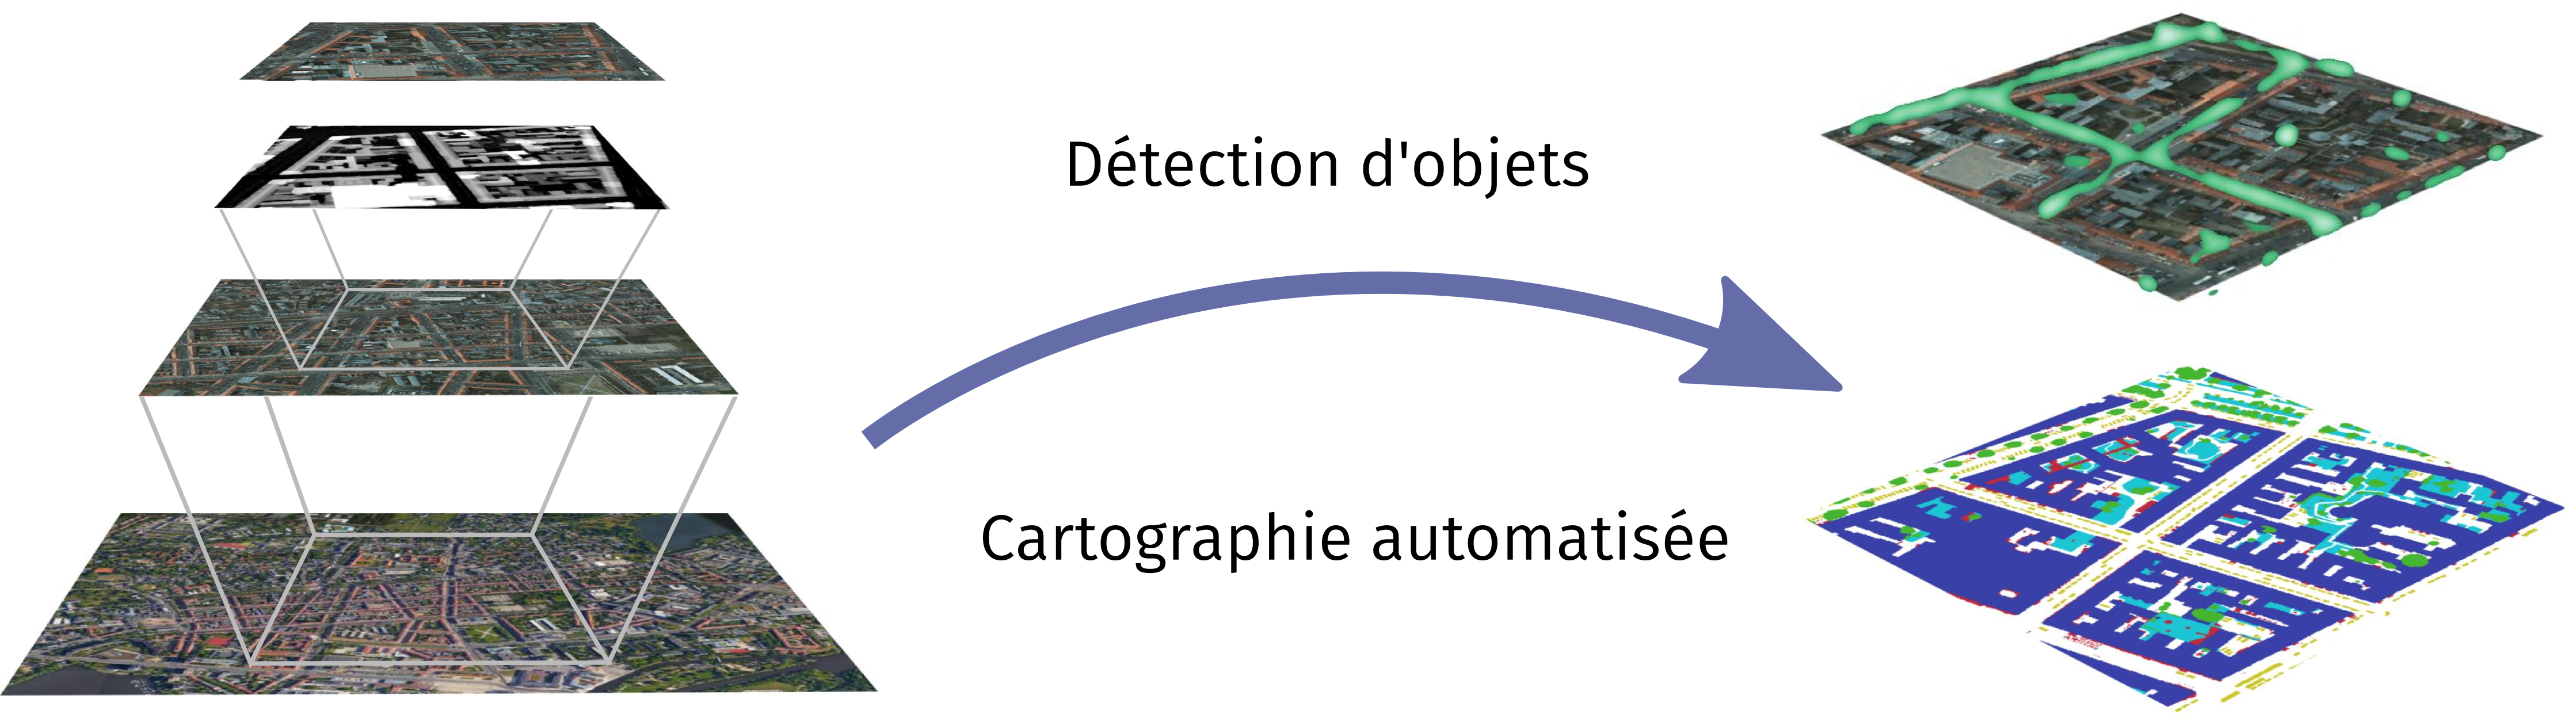
\includegraphics[width=\textwidth]{semantic_mapping}
	\caption{Cartographie automatisée d'images aériennes}
	\label{fig:semantic_mapping}
\end{figure}

En particulier, ce chapitre s'intéresse à la cartographie d'images aériennes à trois canaux, \gls{RVB} ou \gls{IRRV}, en très haute résolution ($<50cm$). L'objectif étant d'étudier la possibilité d'appliquer des méthodes d'apprentissage profond utilisées en vision par ordinateur classique aux images de télédétection, nous nous intéressons dans un premier temps à des images présents des caractéristiques proches des images multimédia\,: résolution élevée et espace de couleur \gls{RVB} ou assimilé, acquises par des appareils photo traditionnels.

En l'occurence, nous souhaitons pouvoir réaliser automatiquement une cartographie sémantique à partir des images, c'est-à-dire associer chaque zone de l'image à une classe d'intérêt thématique (\cref{fig:semantic_mapping}). La tâche à réaliser est donc formellement décrite de la façon suivante\,: compte-tenu d'une image $I$ de dimensions $(w\times{}h)$ et d'un ensemble de classes d'intérêts numérotées de $1$ à $n$ on souhaite associer chaque pixel de l'image $I_{i,j}$ à une classe $k_{i,j} \in \{1..n\}$.

Autrement dit, on cherche à approximer la fonction $f$ telle que\,:
$$\forall (i,j) \in \{1\dots{}w\}\times\{1\dots{}h\} f(I_{i,j}) = k_{i,j}~.$$

Il s'agit d'un problème d'apprentissage automatique de classification. Compte-tenu du fait que l'on travaille sur des images et que les pixels $I_{i,j}$ sont liés spatialement entre eux, on parle habituellement de segmentation sémantique. En effet, l'image ainsi classifiée pourra se représenter sous la forme d'une carte, dans laquelle les pixels sont regroupables par région en fonction de leur classe sémantique.

Afin d'approximer $f$, il est possible de distinguer deux étapes dans le processus de classification de données. La première étape, dite d'extraction de caractéristiques, consiste à transformer la donnée pour la projeter dans un espace de représentation adapté. La seconde consiste à la classification à proprement parler, c'est-à-dire à la séparation de l'espace ainsi formé en sous-ensemble disjoints.

Par exemple, dans le cas d'une machine à vecteur de support linéaire, la classification s'effectue en déterminant les hyperplans permettant de séparer au mieux les données. L'espace de représentation doit donc être, si possible, linéairement séparable. Il s'agit alors de trouver des caractéristiques (c'est-à-dire une projection) adaptées

\subsection{Classification par région}

\subsubsection{Approches pixelliques}

Une acquisition d'observation de la Terre est caractérisée par sa résolution spatiale. Celle-ci détermine l'unité de surface minimale au sein laquelle il devient impossible de séparer deux observations. Dans le cas d'une image, cette résolution en unité de longueur par pixel. Ainsi, une image à résolution de $10m/px$ est un ensemble d'observations, chacune effectuée sur une surface de $10\times10$m. De fait, en traitement d'images de télédétection, le pixel est l'unité atomique de surface. Par conséquent, une mesure pour 1 pixel est la mesure la plus pure disponible. Sans toutefois prétendre qu'une observation sur un pixel ne souffre pas de problèmes de mélanges (en fonction des objets d'intérêt, un pixel peut mélanger plusieurs classes hétérogènes), le pixel représente la mesure la plus fine disponible.

En première approche, il semble raisonnable de traiter le problème de cartographie comme un problème de classification des pixels. Pour ce faire, il est dans un premier temps nécessaire d'extraire des attributs du pixel. Dans le cas d'une image multispectrale, cela peut par exemple être la proportion de lumière réfléchie dans chacune des longueurs d'onde mesurées. Mais il est également possible d'y ajouter d'autres attributs : la valeur moyenne de l'intensité lumineuse ou les observations voisines. Une fois l'extraction d'attributs effectuée, il est possible de réaliser une classification.

L'avantage de cette méthode est qu'elle garantit une résolution identique à celle de la donnée.

Le premier inconvénient est que cette méthode est particulièrement susceptible au bruit. En effet, la classification s'effectuant pixel à pixel, la nature des pixels voisins n'est pas forcément prise en compte. Toutefois, les objets géographiques considérés s'étendent bien souvent sur plusieurs pixels et possèdent des propriétés géométriques particulières de connexité et de convexité. Ainsi, un pixel particulier soumis à un bruit extrême (suite à une défaillance du capteur ou à un matériau particulier), celui risque d'être mal classé de manière isolée, alors que son appartenance à une région particulière aurait pu permettre de contourner cette erreur en se basant sur des critères d'homogénéité. Ainsi la classification pixellique tend à produire des cartes exhibant un comportement de bruit poivre-et-sel.

Le second inconvénient est que le nombre de pixels croît quadratiquement avec la taille de l'image à traiter. Or, les tailles d'images considérées en télédétection peuvent rapidement conduire à devoir traiter des millions de pixels. Le problème de classification peut alors devenir intraitable sur ces images, alors que les capteurs tendent justement à s'améliorer en résolution. En particulier, la litérature s'étant intéressée à ces approches ne traite que d'images de tailles réduites~\cite{nogueira_learning_2016}, notamment dans le cadre de l'imagerie hyperspectrale~\cite{fauvel_advances_2013}.

\subsubsection{Approches par région}

\begin{figure}
\resizebox{\textwidth}{!}{%
\documentclass{standalone}
\usepackage[utf8]{inputenc}
\usepackage[T1]{fontenc}
\usepackage{tikz}
%%%%%%%%%%%%%%%%%%%%%%%%%%%%%%%%%%%%%%%%
%           Commandes perso            %
%%%%%%%%%%%%%%%%%%%%%%%%%%%%%%%%%%%%%%%%

%% Figures centrées, et en position 'here, top, bottom or page'
\newenvironment{figureth}{%
		\begin{figure}[htbp]
			\centering
	}{
		\end{figure}
		}


%% Tableaux centrés, et en position 'here, top, bottom or page'
\newenvironment{tableth}{%
		\begin{table}[htbp]
			\centering
			%\rowcolors{1}{coleurtableau}{coleurtableau}
	}{
		\end{table}
		}

%% Sous-figures centrées, en position 'top'
\newenvironment{subfigureth}[1]{%
	\begin{subfigure}[t]{#1}
	\centering
}{
	\end{subfigure}
}

\newcommand{\citationChap}[2]{%
	\epigraph{\og \textit{#1} \fg{}}{#2}
}

%% On commence par une page impaire quand on change le style de numérotation de pages
\let\oldpagenumbering\pagenumbering
\renewcommand{\pagenumbering}[1]{%
	\cleardoublepage
	\oldpagenumbering{#1}
}

%% Légende du dataset ISPRS
\newcommand\isprslegende{
Légende\,: \textcolor{Black}{blanc}\,: routes, \textcolor{Blue}{bleu}\,: bâtiments, \textcolor{Cerulean}{cyan}\,: végétation basse, \textcolor{OliveGreen}{vert}\,: arbres, \textcolor{Dandelion}{jaune}\,: véhicules, \textcolor{BrickRed}{rouge}\,: autre.
}

%% Dessiner des réseaux de neurones avec Tikz
\newcommand{\convlayer}[9]{%{h}{w}{d}{name}{color}{x}{y}{z}%{note w}{note h}{note d}
   \def\h{#1}
   \def\w{#2}
   \def\d{#3}
   \def\name{#4}
   \ifthenelse {\equal{#5} {}} {\def\col{white}} {\def\col{#5}}
   \def\x{#6}
   \ifthenelse {\equal{#7} {}} {\def\y{0}} {\def\y{#7}}
   \ifthenelse {\equal{#8} {}} {\def\z{0}} {\def\z{#8}}
   % ne faites pas ça chez vous !
   \ifthenelse {\equal{#9} {}} {\convlayercontinued{}{}{}} {\convlayercontinued#9}
}

\newcommand\convlayercontinued[3]{
   \def\notew{#1}
   \def\noteh{#2}
   \def\noted{#3}
   \coordinate (A) at (\x-\d/2,  \y-\h/2, \z-\w/2);
   \coordinate (B) at (\x-\d/2,  \y-\h/2, \z+\w/2);
   \coordinate (C) at (\x-\d/2,  \y+\h/2, \z+\w/2);
   \coordinate (D) at (\x-\d/2,  \y+\h/2, \z-\w/2);
   \coordinate (E) at (\x+\d/2,  \y-\h/2, \z-\w/2);
   \coordinate (F) at (\x+\d/2,  \y-\h/2, \z+\w/2);
   \coordinate (G) at (\x+\d/2,  \y+\h/2, \z+\w/2);
   \coordinate (H) at (\x+\d/2,  \y+\h/2, \z-\w/2);

    \draw [draw opacity=0.3, fill opacity=0.8, fill=\col!60!white] (A) -- (B) -- (C) -- (D) -- cycle;
    \draw [draw opacity=0.3, fill opacity=0.8, fill=\col!60!white] (A) -- (B) -- (F) -- (E) -- cycle;
    % Face haut
    %\draw [left color=\col!60!white, right color=\col!80!white, shading=axis, shading angle=180] (C) -- (D)  -- (H) -- (G) -- cycle;
    \draw [fill opacity=0.9, fill=\col!70!white] (C) -- node[rotate=45,above] {\small \name} (D) -- (H) -- (G) -- cycle;
    %\draw [fill opacity=0.9, fill=\col!70!white] (C) -- (D) -- node[above] {\small \name} (H) -- (G) -- cycle;
    % Face droite
    \draw [fill opacity=0.9, fill=\col!60!white] (E) -- node[pos=0.75,rotate=45,below] {\scriptsize \notew} (F) -- (G) --  (H) -- cycle;
    % Face avant
    %\draw [shading=axis, left color=\col!60!white, right color=\col!40!white, shading angle=-45] (B) -- node[above,rotate=90] {\scriptsize \noteh} (C) -- (G) -- (F) -- node[below] {\scriptsize \noted}  cycle;
    \draw [fill opacity=0.9, fill=\col!50!white] (B) -- node[above,rotate=90] {\scriptsize \noteh} (C) -- (G) -- (F) -- node[below] {\scriptsize \noted}  cycle;
}

\newcommand{\fclayer}[8]{%{h}{w}{name}{color}{x}{y}{z}
   \def\h{#1}
   \def\w{#2}
   \def\name{#3}
   \ifthenelse {\equal{#4} {}} {\def\col{white}} {\def\col{#4}}
   \def\x{#5}
   \def\y{#6}
   \def\z{#7}
   \def\note{#8}
   \coordinate (A) at (\x-\w/2,  \y-\h/2, \z);
   \coordinate (B) at (\x+\w/2,  \y-\h/2, \z);
   \coordinate (C) at (\x+\w/2,  \y+\h/2, \z);
   \coordinate (D) at (\x-\w/2,  \y+\h/2, \z);

   \pgfmathparse{4*\w}\let\boxwidth\pgfmathresult
    \draw [fill=\col] (A) -- node[below,text width=\boxwidth cm,align=center] {\scriptsize \note} (B) -- (C) -- (D) -- cycle;

    \node (N) at ($(A)!0.5!(B)+(0,-1,0)$) {\name};
}

\newcommand{\alexnet}[4]{%{scale}{x}{y}{z}
  \def\scale{#1}
  \def\alexx{#2}
  \def\alexy{#3}
  \def\alexz{#4}


  \def\coblue{blue!50!white}
  \def\fcgrey{gray!50!white}

  \convlayer{1.3*\scale}{1.3*\scale}{0.02*\scale}{Image}{\coblue}{\alexx}{\alexy}{\alexz}{{227}{227}{3}}
  \convlayer{1.1*\scale}{1.1*\scale}{0.08*\scale}{Conv1}{\coblue}{\alexx+0.7*\scale}{\alexy}{\alexz}{{55}{55}{96}}
  \convlayer{0.7*\scale}{0.7*\scale}{0.5*\scale}{Conv2}{\coblue}{\alexx+1.5*\scale}{\alexy}{\alexz}{{27}{27}{256}}
  \convlayer{0.5*\scale}{0.5*\scale}{0.8*\scale}{Conv3}{\coblue}{\alexx+2.6*\scale}{\alexy}{\alexz}{{13}{13}{384}}
  \convlayer{0.5*\scale}{0.5*\scale}{0.8*\scale}{Conv4}{\coblue}{\alexx+3.8*\scale}{\alexy}{\alexz}{{13}{13}{384}}
  \convlayer{0.5*\scale}{0.5*\scale}{0.5*\scale}{Conv5}{\coblue}{\alexx+4.8*\scale}{\alexy}{\alexz}{{13}{13}{256}}
  \fclayer{\scale}{0.1*\scale}{FC1}{\fcgrey}{\alexx+5.4*\scale}{\alexy}{\alexz}{4096}
  \fclayer{\scale}{0.1*\scale}{FC2}{\fcgrey}{\alexx+5.7*\scale}{\alexy}{\alexz}{4096}
  \fclayer{\scale}{0.1*\scale}{FC3}{\fcgrey}{\alexx+6.0*\scale}{\alexy}{\alexz}{1000}
}

\newcommand{\imagelayer}[7]{%{width}{x}{y}{z}{path}{text_up}{text_down}
    \pgfmathparse{#1}\let\w\pgfmathresult
    \begin{scope}[canvas is yz plane at x=#2]
     \node[transform shape] (source) at (#3, #4) {\includegraphics[angle=-90,width=\w cm]{#5}};
    \end{scope}
     \node [transform shape, rotate=45, above] at (source.east) {#6};
     \node [transform shape, rotate=45, below] at (source.west) {\scriptsize{#7}};
}

\def\fourier{\mathcal{F}}

\newcommand{\lightspectrum}{%
\pgfplotsset{
    % this *defines* a custom colormap ...
    colormap={slategraywhite}{color(0cm)=(red); color(1cm)=(red); color(2cm)=(red); color(3cm)=(red); color(4cm)=(orange); color(5cm)=(yellow); color(6cm)=(green); color(7cm)=(blue); color(8cm)=(blue); color(9cm)=(purple); color(10cm)=(purple); color(12cm)=(black)}
}
\node at (1.5, 2.7) {\small 1mm};
\node at (4, 3) {Infrarouge};
\node at (7.75, 2.7) {\small 800nm};
\node at (9, 3) {Visible};
\node at (10.5, 2.7) {\small 400nm};
\node at (12, 3) {Ultraviolet};
\node at (13.5, 2.7) {\small 10nm};
\draw[->] (1, 2.5) -- (14, 2.5);
\begin{axis}[hide axis,width=16cm,height=4cm,colormap name=slategraywhite]
\addplot[domain=20:1000,samples=1500,ultra thick, point meta=x*x,mesh]{sin(x*x/80)};
\end{axis}
}

% Union généralisée
\newcommand{\wbigcup}{\mathop{\bigcup}\displaylimits}

\newcommand{\res}[2]{#1 {\footnotesize $\pm$ #2}}
\newcommand{\bres}[2]{\textbf{#1} {\footnotesize $\pm$ #2}}
\newcommand{\bbres}[2]{\res{\textit{#1}}{#2}}

\newcommand{\drawkernel}[9]{
\begin{tikzpicture}
	\draw[step=1cm,gray!50!white,very thin] (0,0) grid (3,3);
	\kernelnode{0.5}{0.5}{#1};
	\kernelnode{0.5}{1.5}{#2};
	\kernelnode{0.5}{2.5}{#3};
	\kernelnode{1.5}{0.5}{#4};
	\kernelnode{1.5}{1.5}{#5};
	\kernelnode{1.5}{2.5}{#6};
	\kernelnode{2.5}{0.5}{#7};
	\kernelnode{2.5}{1.5}{#8};
	\kernelnode{2.5}{2.5}{#9};
\end{tikzpicture}
}

\newcommand{\kernelnode}[3]{%{x}{y}{value}
	\ifthenelse{\equal{#3}{0}}{
		\def\kcolor{gray}
	}{
		\def\kcolor{black}
	}
	\node[\kcolor] at (#1, #2) {#3};
}

\newcommand{\chapsummary}[1]{
\section*{Résumé du chapitre :}
\parbox{0.9\linewidth}{
\setlength{\parindent}{4ex}
#1}
}

\newcommand{\eqname}[1]{\tag*{\small (#1)}}

\begin{document}

\begin{tikzpicture}[]
\usetikzlibrary{3d}
\usetikzlibrary{calc}
\usetikzlibrary{arrows.meta, bending}

\coordinate (input) at (-5.5,0);
\coordinate (seg) at (0,0);
\coordinate (patches) at (5, 0);
\coordinate (net) at (12, 0);
\coordinate (features) at (18, 0);
\coordinate (classifier) at (21, 0);
\coordinate (map) at (26, 0);

\node (in_fig) at (input) {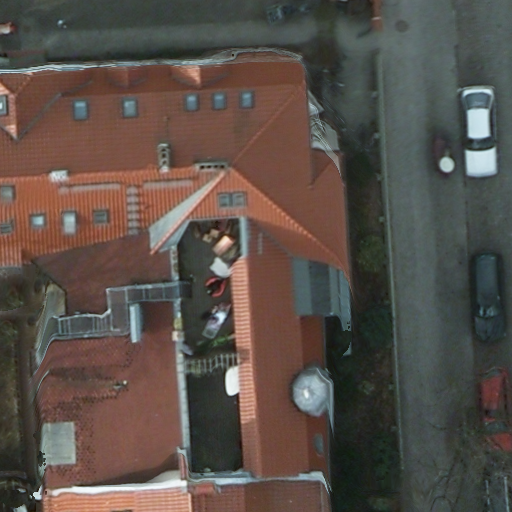
\includegraphics[width=3cm]{orthohr_rgb}};
\node at ($ (input) - (0,2)$) {Image initiale};

\node (seg_fig) at (seg) {\includegraphics[width=3cm]{orthohr_rgb_slic}};
\node at ($ (seg) - (0,2)$) {Image segmentée};

\draw[->] (in_fig.east) to node[above]{\footnotesize segmentation} (seg_fig.west);

\node (large) at ($ (patches)+(0,2.5)$) {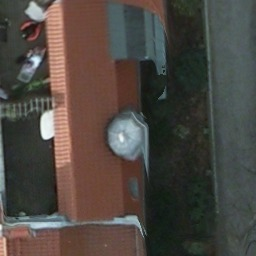
\includegraphics[width=2cm]{large}};
\node (medium) at (patches) {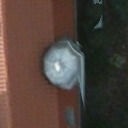
\includegraphics[width=2cm] {medium}};
\node (ndsm) at ($ (patches)-(0,2.5) $) {\includegraphics[width=2cm]{ndsm}};

\draw ($(seg_fig.east)-(1.2,0.8)$) edge[in=180,out=0,->] node[right]{\footnotesize{contexte}} (medium.west);
\draw ($(seg_fig.east)-(1.2,0.8)$) edge[in=180,out=0,->] node[right]{\footnotesize{contexte}}(large.west);
\draw ($(seg_fig.east)-(1.2,0.8)$) edge[in=180,out=0,->] node[right]{\footnotesize{MNS}} (ndsm.west);

\node[align=center] at ($ (patches)-(0,4.5) $) {Entrées multi-sources\\ et multi-échelles};

\node (net_fig) at (net) {\includegraphics[width=8cm]{../alexnet}};
\node at ($ (net) - (0,2)$) {CNN pré-entraîné};

\draw (large.east) edge[in=180,out=0,->] (net_fig.west);
\draw (medium.east) edge[in=180,out=0,->] (net_fig.west);
\draw (ndsm.east) edge[in=180,out=0,->] (net_fig.west);

\coordinate (A) at ($ (features)+(0,-3,-0.5)$);
\coordinate (B) at ($ (features)+(0,3,-0.5)$);
\coordinate (C) at ($ (features)+(0.5,3,-0.5)$);
\coordinate (D) at ($ (features)+(0.5,-3,-0.5)$);
\coordinate (E) at ($ (features)+(0,-3,0)$);
\coordinate (F) at ($ (features)+(0,3,0)$);
\coordinate (G) at ($ (features)+(0.5,3,0)$);
\coordinate (H) at ($ (features)+(0.5,-3,0)$);

\coordinate (I) at ($ (E)!0.33!(F)$);
\coordinate (J) at ($ (E)!0.66!(F)$);
\coordinate (K) at ($ (H)!0.33!(G)$);
\coordinate (L) at ($ (H)!0.66!(G)$);
\coordinate (M) at ($ (D)!0.33!(C)$);
\coordinate (N) at ($ (D)!0.66!(C)$);

\def\grey{gray!40!white}
\draw[fill=\grey] (A) -- (B) -- (C) -- (D) -- cycle;
\draw[fill=\grey!60!white] (E) -- (F) -- (G) -- (H) -- cycle;
\draw[fill=\grey] (B) -- (C) -- (G) -- (F) -- cycle;
\draw[fill=\grey] (C) -- (D) -- (H) -- (G) -- cycle;
\draw[dotted,thick] (I) -- (K) -- (M);
\draw[dotted,thick] (J) -- (L) -- (N);
\node[align=center] at ($ (features) - (0,4.5)$) {Caractéristiques\\ profondes};

\draw (net_fig.east) edge[out=0,in=180,->] ($(I)!0.5!(E)$);
\draw (net_fig.east) edge[out=0,in=180,->] ($(J)!0.5!(F)$);
\draw (net_fig.east) edge[out=0,in=180,->] ($(F)!0.5!(E)$);

\coordinate (c_A) at ($ (classifier) + (-1,1.5)$);
\coordinate (c_B) at ($ (classifier) + (-1,-1.5)$);
\coordinate (c_C) at ($ (classifier) + (1,-1.5)$);
\coordinate (c_D) at ($ (classifier) + (1,1.5)$);
\coordinate (c_top) at ($(c_A)!0.5!(c_D)$);
\coordinate (c_bottom) at ($ (c_B)!0.5!(c_C)$);
\filldraw[fill=yellow!50!white] (c_A) rectangle (c_C);


\newcommand\children[3]{
\coordinate (#1_c1) at ($(#1)!0.5!(#2)$);
\filldraw[fill=black] (#1_c1) circle (0.08);
\draw (#1) -- (#1_c1);
\coordinate (#1_c2) at ($(#1)!0.5!(#3)$);
\filldraw[fill=black] (#1_c2) circle (0.08);
\draw (#1) -- (#1_c2);
}

\coordinate (c_center) at ($(c_A)!0.5!(c_C)$);
\coordinate (c_center) at ($(c_center)!0.75!(c_top)$);
\filldraw[fill=black] (c_center) circle (0.1);
\coordinate (n1) at ($(c_center)!0.25!(c_B)$);
\filldraw[fill=black] (n1) circle (0.08);
\draw (c_center) -- (n1);
\coordinate (n2) at ($(c_center)!0.25!(c_C)$);
\filldraw[fill=black] (n2) circle (0.08);
\draw (c_center) -- (n2);

\children{n2}{c_bottom}{c_C}
\children{n2_c2}{c_bottom}{c_C}

\children{n1}{c_B}{c_bottom}
\children{n1_c1}{c_B}{c_bottom}

\node at ($(classifier) - (0,2)$) {Classifieur};

\draw ($(G)!0.5!(H)$) edge[in=180,out=0,->]  ($(c_A)!0.5!(c_B)$);

\node (map_fig) at (map) {\includegraphics[width=3cm]{gt_boundaries}};
\node at ($(map) - (0,2)$) {Carte sémantique};

\draw ($(c_C)!0.5!(c_D)$) edge[in=180,out=0,->] node[above]{\footnotesize prédiction} (map_fig.west);

\end{tikzpicture}

\end{document}

}
\caption{Segmentation sémantique par régions d'une image aérienne. Chaque région de l'image segmentée est classifiée à partir de caractéristiques profondes extraites d'un réseau convolutif pré-entraîné.}
\label{fig:framework}
\end{figure}

Compte-tenu de l'explosion du coût calculatoire des classifications pixelliques sur des images \gls{HR}, \gls{THR} et \gls{EHR}, plusieurs travaux se sont penchés sur des approches considérant d'autres découpages de l'image que la grille de pixels. En particulier, il est envisageable de regrouper des pixels similaires dans des régions homogènes. La similarité peut alors uniquement se fonder sur des critères statistiques liées aux valeurs des pixels, ou à des critères sémantiques. Dans le premier cas, on parlera de ``superpixels'' et dans le second cas de ``segmentation''.

L'avantage de ces méthodes est qu'elles permettent de regrouper des pixels d'apparence similaire dans une même région. Or, on peut raisonnablement s'attendre à ce que des pixels spatiallement et spectralement proches possèdent la même sémantique, c'est-à-dire que l'on puisse les associer à la même classe d'intérêt. Dans ce cas, plutôt que de réaliser la classification pixel par pixel, il est possible de ne réaliser qu'une seule extraction d'attributs pour l'ensemble de la région homogène et de ne faire qu'une unique prédiction. Ainsi, dans le cas d'une image de dimensions $1500\times1500$ segmentée en $20 000$ régions, on peut alors cartographier l'image en classifiant $20 000$ régions plutôt qu'en classifiant \nombre{2250000} pixels, soit ungain en temps de calcul d'un facteur $112$ (segmentation exclue).

De nombreux algorithmes de segmentation ont été proposés, aussi bien dans la communauté télédétection que dans la communauté vision par ordinateur. Ces algorithmes de segmentation viennent partitionner l'ensemble des pixels de façon non-supervisée. Une fois ce partitionnement effectué, il est possible d'extraire des attributs pour chaque région et d'entraîner un classifieur de la façon usuelle, l'inférence se faisant de façon analogue. Ce procéde est illustré dans la~\cref{fig:framework}.

L'avantage principal de ces méthodes est de grandement réduire la complexité calculatoire. Notamment, lorsque l'image augmente de résolution spatiale, de nombreuses régions conservent leur homogénéité et il est ainsi très avantageux de les conserver regroupées\,: l'augmentation de la résolution ne nécessite pas obligatoirement une évolution quadratique du nombre de régions segmentées. Ces approches ont ainsi été utilisées avec succès dans le cadre de la segmentation sémantique d'images aériennes \gls{THR}~\cite{lagrange_benchmarking_2015,vargas_superpixel-based_2014}.

On peut noter que traiter l'image par une fenêtre glissante ou même par une grille de pixels correspond à des cas particuliers de classification par région.

\subsection{Algorithmes de segmentation}

Il existe de nombreux algorithmes de segmentation d'image non-supervisés. Les approches les plus anciennes traitent des images monochromes en niveaux de gris tandis que les plus récentes peuvent travailler dans espaces couleurs comme \gls{RVB}, hue-saturation-intensité ou encore l'espace \gls{LAB}.

Une première famille de segmentation traite l'image sous la forme d'un graphe. Formellement, les pixels sont représentés par les n\oe{}uds du graphe dont les arêtes représentent les relations de similarité entre pixels voisins. La construction des régions de l'image se fait alors en agglomérant les noeuds du graphe en fonction des arêtes qui les relient. C'est sur ce principe que fonctionne l'algorithme de segmentation \gls{FH}~\cite{felzenszwalb_efficient_2004}, qui segmente l'image en calculant un arbre couvrant de poids minimal, mais aussi l'algorithme \emph{Normalized Cuts}~\cite{shi_normalized_2000} qui aborde le problème sous l'angle du partitionnement de graphe. C'est également l'approche utilisée pour les algorithmes à base de marche aléatoire sur le graphe de l'image, soit pour la minimisation d'une fonction entropie pour l'algorithme \gls{ERS}~\cite{liu_entropy_2011}, soit pour la résolution d'équation de diffusion~\cite{grady_random_2006}.

Une seconde approche, particulièrement populaire dans la littérature récente, utilise des algorithmes itératifs de \emph{clustering} (partitionnement de données) pour la segmentation. Ce procédé a engendré deux grandes familles de segmentations dites \og superpixels \fg. La première est dérivée de l'algorithme \gls{SLIC}~\cite{achanta_slic_2010}. Cet algorithme projette les pixels dans un espace de représentation couleur-$(x,y)$ de dimension 5 et utilise un algorithme de partitionnement itératif dérivé des $k$-moyennes. \gls{SLIC} initialise un nombre de centres déterminé par l'utilisateurs sur une grille régulière, puis met à jour itérativement ceux-ci en absorbant les pixels voisins de la frontière des régions segmentées. Cette méthode vu naître plusieurs variantes, dont le \emph{Preemptive SLIC}~\cite{neubert_compact_2014}, plus rapide, l'algorithme \gls{LSC}~\cite{li_superpixel_2015} intégrant des contraintes globales en plus de la mise à jour itérative locale et l'algorithme \gls{SCALP}~\cite{giraud_robust_2018}. \gls{SCALP} interdit l'appartition de superpixels de forme non-régulière dans l'image en considérant l'ensemble des pixels sur le chemin entre le barycentre du superpixel et celui à ajouter. En outre, \gls{SCALP} prend en entrée le résultat d'un algorithme de détection de contours afin de renforcer l'adhérence des superpixels aux bordures des objets.
La deuxième grande famille d'algorithmes de segmentation superpixels se base sur le principe des $k$-médoïdes. En particulier, il s'agit de projeter les pixels dans un espace non-euclidien de dimension 5 (généralement RVB-$(x,y)$) puis de réaliser le partitionnement en cherchant le mode dominant local de chaque voisinage, c'est-à-dire la médoïde. Cette approche a notamment utilisée pour les algorithmes \emph{Mean Shift}~\cite{comaniciu_mean_2002} et \emph{Quickshift}~\cite{vedaldi_quick_2008}.
Plusieurs autres algorithmes utilisent également des approches itératives de partitionnement. L'algorithme \gls{SEEDS}~\cite{bergh_seeds:_2012} définit ainsi des blocs de pixels capables d'échanger des éléments le long de leur frontière afin de maximiser une fonction d'énergie dépendant des histogrammes de couleurs. \gls{SEEDS} utilise une optimisation par \emph{hill-climbing} afin de faire converger itérativement les blocs vers une segmentation stable. Enfin, il existe également des algorithmes itératifs convergeant vers une segmentation à partir de la méthode des surfaces de niveau, comme l'algorithme de Chan-Vese~\cite{chan_active_1999} dérivé des contours actifs ou l'algorithme \emph{TurboPixel}~\cite{levinshtein_turbopixels:_2009} se basant à la fois sur la courbure et le gradient locaux de l'image.

Pour la segmentation d'images en niveaux de gris, l'approche morphologique \emph{watershed} (ou segmentation par ligne de partage des eaux)~\cite{beucher_morphological_1993} est particulièrement populaire. \emph{Watershed} considère l'image comme une carte d'élévation dans laquelle est simulée l'élévation du niveau de l'eau. Initialement, l'eau s'écoule depuis un certain de nombre de sources positionnées sur des marqueurs, qui peuvent être insérés manuellement ou calculés automatiquement, par exemple aux extrema locaux du gradient de l'image. L'eau remplit alors le relief topographique et le niveau est artificiellement augmenté. Lorsque deux sources se rencontrent, un barrage virtuel est érigé à leur ligne de démarcation, établissant ainsi une des frontières de la segmentation. L'algorithme s'arrête lorsque toute l'image a été inondée. Le choix des marqueurs initiaux de \emph{watershed} est critique pour la qualité de la segmentation et notamment à la régularité des régions produites. Une version dite compacte a été proposée~\cite{neubert_compact_2014} afin de rendre \emph{watershed} robuste à l'initialisation, en la rendant plus proche de~\gls{SLIC}. L'approche morphologique peut également être utilisée dans le cadre des contours actifs, notamment dans une variante de l'algorithme Chan-Vese~\cite{chan_active_1999} utilisant les contours actifs morphologiques~\cite{marquez-neila_morphological_2014}.

Enfin, des algorithmes spécifiques au traitement d'images télédétection, notamment radar et multispectrales, ont été proposées dans la littérature. Ces segmentation prennent notamment en compte des aspects multi-échelles avec pour objectif final l'analyse d'image orientée objet. Ainsi, l'algorithme \gls{MRS}~\cite{baatz_multiresolution_2000} est une méthode populaire de segmentation d'images de télédétection, notamment grâce à son implémentation dans le logiciel eCognition\copyright. \gls{MRS} se focalise sur l'identification d'objets saillants dans l'image sur lesquels définir une segmentation. \gls{MRS} utilise une approche par croissance de régions selon un critère d'homogénéité spectrale défini de façon heuristique. \gls{MRS} exécute une segmentation à plusieurs échelles et choisit de conserver ou de fusionner les régions les plus fines selon un critère de similarité.
L'algorithme \gls{HSEG}~\cite{tilton_best_2012} quant à lui produit un segmentation hiérarchique multi-échelles. En effet, \gls{HSEG} produit plusieurs segmentations, organisées sous forme d'arbre\,: une région de l'échelle la plus grande est sous-divisée en plusieurs régions, elles-mêmes pouvant être divisée récursivement. \gls{HSEG} utilise une approche par croissance de régions dans laquelle les pixels proches sont itérativement fusionnés à moins de vérifier un critère spécifique de dissimilarité. Des régions voisines peuvent ensuite être elles-même fusionnées en cas d'homogénéité, afin de produire une segmentation hiérarchique à une échelle plus faible.

\begin{figure}[t]
\foreach \picname\path in {Image originale/fox,SLIC/fox_slic,Quickshift/fox_quickshift,Algorithme MRS/fox_ecognition,FH/fox_felzenszwalb,Watershed/fox_watershed}
{
\begin{subfigure}{0.33\textwidth}
    \includegraphics[width=\textwidth]{\path}
    \includegraphics[width=\textwidth]{\path_patchwork}
    \caption*{\picname}
\end{subfigure}%
}
\caption{Segmentations d'une image naturelle. Certains algorithmes produisent des régions faiblement régulières, mais capturant mieux les détails de l'image.}
\label{fig:fox_segmentation}
\end{figure}

\begin{figure}[t]
\foreach \picname\path in {Image originale/potsdam,SLIC/potsdam_slic,Quickshift/potsdam_quickshift,Algorithme MRS/potsdam_ecognition,FH/potsdam_felzenszwalb,Watershed/potsdam_watershed}
{
\begin{subfigure}{0.33\textwidth}
    \includegraphics[width=\textwidth]{\path}
    \includegraphics[width=\textwidth]{\path_patchwork}
    \caption*{\picname}
\end{subfigure}%
}
\caption{Segmentations d'une image aérienne. Selon l'algorithme appliqué, les voitures sont plus ou moins bien segmentées.}
\label{fig:potsdam_segmentation}
\end{figure}


\subsection{Choix de la méthode de segmentation}

Face à la profusion de méthodes de segmentation existantes vient la question du choix de celle le plus adapté pour l'apprentissage statistique de modèles de classification. Deux critères sont à prendre en compte\,: quels pré-traitements est-il nécessaire d'appliquer à l'image, et quelle segmentation semble respecter au mieux les propriétés spatiales de l'image ?


\subsubsection{Pré-traitement de l'image}
La plupart des algorithmes de segmentation recommandent de traiter au préalable l'image à segmenter en lui appliquant un flou gaussien plus ou moins prononcé. Ce prétraitement se justifie en cela qu'il adoucit les bordures et réduit l'influence du bruit dans l'image, facilitant la segmentation. Empiriquement, pour des images aériennes, un léger flou gaussien suffit à obtenir des segmentations superpixels cohérentes. L'application de ce flou ne sert qu'à la segmentation, et peut bien entendu être abandonnée au moment de la classification.

La segmentation se fait dans la plupart des cas dans l'espace de couleurs LAB. Cet espace de couleurs est conçu pour refléter la vision humaine, en particulier la courbe de réponse de l'oeil humain aux variations de couleurs, qui est logarithmique plutôt que linéaire. Cependant, cela nécessite de s'interroger sur la pertinence d'une telle conversion lorsque les trois canaux des images aériennes ne sont pas \gls{RVB}, mais \gls{IRRV} par exemple. En pratique, cela ne semble pas poser de problèmes, mais ces techniques de segmentation ne se généraliseront donc pas nécessairemment telles quelles pour des images dont la structure est différente du \gls{RVB} traditionnel, en particulier pour le traitement d'images multispectrales. Seuls les algorithmes \gls{MRS} et \gls{HSEG} ont été conçus avec la télédétection comme application finale.

\subsubsection{Forme et tailles des régions}

Plusieurs analyses préliminaires~\cite{neubert_superpixel_2012,achanta_slic_2012} montrent que les différents algorithmes de segmentation peuvent avoir des propriétés très différentes. Notamment, différents algorithmes ne sont pas robustes aux mêmes perturbations et ne segmentent pas les images de la même façon. Notamment, la plupart des algorithmes de segmentation par partitionnement de graphes tendent à ne pas donner à l'utilisateur de contrôle sur la forme et la compacité des régions segmentées. Un exemple qualitatif de segmentation sur une image naturelle est donné dans la~\cref{fig:fox_segmentation}.

Le premier constat qu'il est possible d'en tirer est que les différentes familles d'algorithmes génèrent des segmentations d'aspect variable. L'algorithme de segmentation \gls{FH} génère par exemple des régions de taille et de forme très hétérogènes. En effet, \gls{FH} n'est pas contraint dans son exploration de l'image, et parvient ainsi à rassembler de très grandes surfaces (notamment des routes) dans une unique région. Ce partitionnement peut ainsi conduire à des régions de quelques pixels quand d'autres recouvrent une large portion de l'image, sans qu'aucun paramètre ne puisse contrôler cette variabilité.

À l'opposé, les méthodes de type superpixels et plus particulièrement les dérivés de \gls{SLIC}, donnent des résultats visuellement réguliers. Cette propriété s'accroît lorsque le paramètre de compacité est augmenté afin de contraindre l'adhérence à la grille. Notamment, il est assez aisé de maintenir les superpixels segmentés par \gls{SLIC} à une taille raisonnable tout en leur laissant une certaine liberté de forme. Quickshift se comporte de manière similaire, bien que les superpixels générées soient nettement plus irréguliers que dans les méthodes dérivées de~\gls{SLIC}, ce qui produit des artefacts dans la segmentation. La segmentation \emph{watershed} compacte présente des caractéristiques très similaires aux méthodes de superpixels, et il est préférable de l'utiliser tant l'approche classique est sensible au choix des marqueurs. Ces analyses sont conformes aux études de la littérature~\cite{neubert_superpixel_2012,achanta_slic_2012}.

Toutefois, l'application finale étant la classification d'images de télédétection, il est intéressant d'étudier le comportement des algorithmes de segmentation sur des données prises à la verticale du sol. Un exemple est illustré dans la~\cref{fig:potsdam_segmentation}. L'algorithme \gls{MRS} semble particulièrement adapté aux images de télédétection. En effet, bien que la segmentation paraisse visuellement chaotique, la composition de l'image est respectée jusque dans les moindres détails. Les algorithmes de type superpixels tendent à faire disparaître les détails, et notamment les véhicules, ce qui peut poser problème pour les approches de modélisation d'objets.

Compte-tenu de cette analyse, nous étudierons en priorité les algorithmes de segmentation prévus pour la télédétection (\gls{HSEG} et \gls{MRS}) ainsi qu'un représentant de chaque grande famille de segmentation\,: Quickshift et \gls{SLIC}. Les approches \emph{watershed} sont écartées compte-tenu de leur forte proximité avec \gls{SLIC}~\cite{neubert_compact_2014} tandis que l'approche \gls{FH} est éliminée de part sa grande variabilité entre régions~\cite{neubert_superpixel_2012}.

\subsection{Extraction de caractéristiques}

Une fois les données acquises et mises en forme, il est nécessaire de choisir une méthode de représentation adaptée à la classification. En particulier, il s'agit de chercher un espace de représentation dans lequel projeter les données, de manière à ce qu'il soit aisé de partitionner l'espace afin d'y séparer les différentes classes. Il existe plusieurs approches envisageables.

\subsubsection{Données brutes}

L'approche naïve consiste à simplement utiliser les données brutes sans transformation particulière (éventuellement une transformation affine pour normaliser les valeurs numériques). Dans ce cas, le classifieur prendra directement en entrée les valeurs des canaux Rouge, Vert et Bleu ou les valeurs d'inensité lumineuses ou de réflectance dans le cas d'une image multispectrale. Toutefois, il est inenvisageable de travailler ainsi sur de grandes images. Une image RVB classique de dimensions $128\times128$ serait décrite par l'ensemble des $128\times128\times3 = 49152$ valeurs qui la compose. Cela ne peut donc que s'appliquer que pour approches pixelliques ou pour des régions de taille très faible. Cette approche est cependant courante pour le traitement de données hyperspectrales~\cite{fauvel_advances_2013,ham_investigation_2005} et multispectrales, y compris \gls{IRRVB}~\cite{dechesne_semantic_2017}.

\subsubsection{Statistiques}

Une approche plus raffinée consiste à extraire un certain nombre de paramètres statistiques liées aux données brutes, comme les valeurs minimales et maximales, les valeurs moyenne et médiane, mais aussi la variance ou les extrema du gradient. Cette méthode a l'avantage de produire un vecteur de caractéristique dont la taille ne dépend pas du nombre de pixels considérés et peut donc s'appliquer sur des régions de taille et forme variables. Toutefois, le choix exact des paramètres à prendre en compte n'est pas trivial. Ainsi, il est possible de s'interroger su la pertinence de prendre les extrema du gradient, de la dérivée seconde, etc. Mais également de savoir s'il est nécessaire de compléter les extrema et la médiane par les différents déciles.

\subsubsection{Indices experts}

Les connaissances physiques a priori sur les données peuvent occasionnellement permette de calculer certains indices aisément interprétables. Par exemple, dans le cas de la présence d'une information concernant l'intensité lumineuse en proche-infrarouge, il est possible de calculer l'indice NDVI, ou l'indice NDWI. L'avantage de ces indices est leur interprétabilité physique\,: l'intensité du NDVI correspond directement à un rapport d'énergie lumineuse réfléchie. Toutefois, la diversité des indices possibles nécessite d'une part une connaissance experte des phénomènes observés et recherchés (impossible de détecter un phénomène que l'on ne saurait pas caractériser physiquement, au moins partiellement) et un effort systématique d'ingiénérie, puisqu'il devient nécessaire d'ajuster la liste d'indices pour chaque problème.

\subsubsection{Histogrammes}

Un moyen de s'affranchir des limitations des données radiométriques pour un pixel consiste à considérer un voisinage autour de celui-ci. Un pixel peut être représenté par la distribution des intensités lumineuses sur un voisinage. Cette distribution peut être représentée de façon discrète sous la forme d'un histogramme. Dans le cas du \gls{RVB}, on parle alors d'histogramme de couleur.

Les histogrammes de couleurs peuvent se généraliser à des images multispectrales ou hyperspectrales de la même façon qu'ils s'appliquent aux images \gls{RVB}. Les histogrammes ainsi conçus ont pour propriétés d'être invariant aux rotations et aux translations locales, mais aussi aux changements d'échelle. Toutefois, ils sont fortement susceptibles aux changements radiométriques induits par l'environnement, comme la variation de la luminosité extérieure. En outre, la discrétisation des valeurs dans l'histogramme ajoute une robustesse au bruit, mais fait perdre la précision des valeurs, notamment dans le cas multispectral où des pics d'absorption caractéristiques peuvent alors disparaître. Pour rendre les histogrammes insensibles au nombre de pixels considérés, il est possible de les normaliser.

Les histogrammes peuvent également se calculer sur les variations d'intensité, auquel cas on parle d'histogrammes de gradient. Sur une image 2D, ces histogrammes peuvent se calculer selon plusieurs directions\,: il s'agit d'\gls{HOG}~\cite{dalal_histograms_2005}. Les \gls{HOG} se rapprochent des descripteurs \gls{SIFT}~\cite{lowe_object_1999}, à la différence qu'ils peuvent se calculer de façon dense sur l'image, et non uniquement sur un ensemble parcimonieux de points d'intérêt.

\subsubsection{Combinaison de caractéristiques}

Il est important de noter que les caractéristiques peuvent se calculer à plusieurs échelles (par exemple en incluant différentes tailles de contexte spatial) et qu'il est possible de combiner plusieurs caractéristiques par simple concaténation. On peut ainsi considérer à la fois les statistiques radiométriques et un histogramme de couleurs.

Une approche courante pour la classification de données multispectrales consiste à combiner pour un même pixel les données radiométriques brutes, les moments statistiques de premier ordre et certains indices bien choisis, comme le NDVI~\cite{dechesne_semantic_2017}. En outre, les caractéristiques sur plusieurs sources d'entrée peuvent être combinées dans un cadre d'apprentissage multi-modal.

\subsection{Modèles statistiques usuels}

Une fois le vecteur de caractéristiques extrait pour un échantillon, celui-ci sert alors d'entrée à un classifieur. Le classifieur est un modèle statistique de décision pouvant prendre plusieurs formes. Cette partie ne traite que des classifieurs sans apprentissage de représentation. En particulier, les réseaux de neurones artificiels profonds seront traités dans la section suivante.

\subsubsection{Arbres de décisions}

Les arbres de décision~\cite{breiman_classification_2017} forment un ensemble de modèles statistiques représentant les variables sous forme de n\oe{}ud intérieur, chaque arête correspondant à un ensemble de valeurs possibles pour la variable associée au n\oe{}ud. L'ensemble des arêtes partant d'un n\oe{}ud donné couvre l'ensemble des valeurs que peut prendre la variable qui lui est associée. Durant la phase d'apprentissage, l'arbre est construit par partionnement récursif, divisant l'ensemble des données en fonction d'une première variable, puis de la seconde et ainsi de suite jusqu'à ce que l'ajout de variable n'améliore plus la prédiction, ou que tous les sous-ensemble aboutissent au même résultat.

Les arbres de décision sont couramment utilisés sous forme de forêts aléatoires~\cite{breiman_random_2001}. Une forêt aléatoire est en réalité un ensemble d'arbres décisions construits à partir de sous-ensembles aléatoires des variables d'entrée. Chaque arbre réalise sa prédiction indépendamment des autres, et la prédiction finale est celle ayant obtenu le plus de voteS.


\subsubsection{Séparateurs à Vaste Marge}

Les \gls{SVM}~\cite{boser_training_1992,cortes_support-vector_1995} sont des classifieurs partionnant l'espace de telle sorte que la distance entre la frontière et l'échantillon le plus proche (la marge) soit maximale. La frontière se représente sous la forme d'un hyperplan dans l'espace des données d'entrée dans le cas du noyau linéaire, ou d'un hyperplan dans un espace de représentation de grande dimension (possiblement infinie).

Dans le cas où la dimension des données d'entrée est de grande taille, le calcul exact des hyperplans à marge maximale n'est pas nécessairement réalisable en temps raisonnable. Dans ce cas, il est possible de faire appel à des algorithmes d'approximation reposant sur une optimisation par descente de gradient~\cite{bottou_large-scale_2010}.

\subsubsection{Gradient boosting}

Le principe du gradient boosting est d'exploiter un ensemble de modèles de prédiction faibles pour les combiner et renforcer leur pouvoir de prédiction. Cette technique a notamment été utilisée dans le cadre des arbres de décision et popularisée dans la méthode dite XGBoost~\cite{friedman_greedy_2001}.

\section{Réseaux de neurones profonds}

\subsection{Réseaux de neurones convolutifs comme extracteurs de caractéristiques}

Jusqu'ici les méthodes d'extraction de caractéristiques que nous avons évoqué ne dépendent pas des données. En effet, il s'agit de méthodes calculatoires qui s'appliquent de la même façon sur des images aériennes ou des images multimédia.

Cependant, l'intérêt majeur de l'apprentissage profond réside dans l'apprentissage des représentations~\cite{bengio_representation_2013,goodfellow_deep_2016}. En effet, à partir des images d'entrées, nous avons vu que les réseaux convolutifs réalisent une extraction de caractéristique. Cette projection dans un espace de représentation est réalisée par les premières couches, qui sont elles-mêmes optimisables. Autrement dit, la représentation apprise est optimisée pour la tâche de classification sur les données d'entraînement.

Il est donc possible de fournir une image à un réseau et de stopper le calcul des activations avant la dernière couche. Les activations ainsi obtenues peuvent se représenter sous la forme d'un vecteur de caractéristiques.

Les caractéristiques ainsi extraites peuvent ensuite être utilisées pour entraîner un classifieur de façon habituelle. Cette approche est similaire au principe de spécialisation d'un réseau par \emph{fine-tuning}. En particulier, il a été montré dans~\cite{razavian_cnn_2014} que l'utilisation des caractéristiques extraites par un réseau pré-entraîné sur le jeu de données ImageNet~\cite{deng_imagenet:_2009} pour entraîner une \gls{SVM} linéaire donnait d'excellents résultats sur la plupart des tâches visuelles.~\cite{razavian_cnn_2014} défend ainsi l'idée qu'il s'agit d'une méthode simple à mettre en \oe{}uvre et qui permet d'obtenir immédiatement des résultats satisfaisants, généralement meilleurs que ceux obtenues avec les caractéristiques classiques (\gls{HOG}, \gls{SIFT}\dots). Il est intéressant de constater que les représentations apprises par les réseaux convolutifs sont généralement de meilleurs points de départ pour l'optimisation que des initialisations aléatoires, même dans le cas de tâches très différentes~\cite{yosinski_how_2014}.

Ces résultats ont été repris et confirmés dans~\cite{penatti_deep_2015,marmanis_deep_2016,lagrange_benchmarking_2015} pour la classification d'images aériennes. En particulier,~\cite{marmanis_deep_2016,penatti_deep_2015} montre qu'il est possible d'utiliser les caractéristiques extraites par un réseau pré-entraîné sur ImageNet pour la classification d'images aériennes et satellitaires, ce qui a été étendu à la segmentation sémantique par région par la suite~\cite{lagrange_benchmarking_2015}. Ce résultat est contre-intuitif dans la mesure où les images de la base ImageNet sont des images multimédia classiques\,: animaux, objets du quotidien, personnes, paysages\dots Toutefois, les caractéristiques apprises sur ces images semblent être en mesure de se généraliser aux images de télédétection. Autrement dit, les filtres convolutifs appris lors d'un entraînement sur ImageNet sont suffisamment génériques pour pouvoir être appliqués dans un grand nombre de tâches visuelles.

\subsubsection{Application à la cartographie sémantique}

À partir des procédés de segmentation et des méthodes de classification décrites précédemment, nous pouvons donc construire un processus complet de segmentation sémantique d'une image aérienne, repris de la~\cref{fig:framework}\,:
\begin{enumerate}
    \item Diviser l'image en sous-régions homogènes à l'aide d'un algorithme de segmentation.
    \item Pour chaque région, extraire des imagettes de dimensions $32\times32$, $64\times64$ et $128\times128$ autour du centroïde de la région.
    \item Extraire les caractéristiques de chaque imagette.
    \item Concaténer les vecteurs résultants dans un unique vecteur de caractéristique.
\end{enumerate}

Les échantillons d'apprentissage ainsi obtenus peuvent être utilisés pour entraîner le classifieur durant la phase d'apprentissage, ou simplement pour la prédiction en phase d'évaluation.

Dans le cas où l'extraction de caractéristiques est réalisée par un réseau convolutif, il est nécessaire de redimensionner l'imagette à la taille requise par le réseau (par exemple, $228\times228$ pour l'architecture AlexNet). Cette nécessité provient de la présence de couches entièrement connectées, qui contraignent la taille de la caractéristique obtenue en sortie de couches convolutives, et donc les dimensions initiales de l'image.

En outre, dans certains cas, la taille du vecteur de caractéristique est particulièrement grande. Pour AlexNet, la caractéristique obtenue est un vecteur de taille $1 000$ pour chaque imagette. Une région donnée génère donc un vecteur de taille $3 000$. Pour rendre l'optimisation de la SVM calculable, ses paramètres sont alors approximés par descente de gradient stochastique, et non calculés de façon exacte.

\subsection{Réseaux de neurones entièrement convolutifs}

On enlève la partie entièrement connectée pour en faire une partie convolutive

Avantage : prédiction spatiale et non plus unidimensionnelle
Avantage : plus de taille fixée d'image
Avantage : on fait automatiquement la classification pixellique !

\subsubsection{Application à la cartographie sémantique}

Nous choisissons ici deux modèles\,: SegNet et ResNet.

De nombreuses architectures de FCN sont disponibles pour la segmentation sémantique. Nous retenons le modèle SegNet~\cite{badrinarayanan_segnet:_2017} (cf. \cref{fig:segnet}) qui présente un équilibre satisfaisant entre précision de la classification et temps de calcul. L'architecture de SegNet est symétrique et permet de replacer précisément les caractéristiques abstraites aux bonnes localisations spatiales. En outre, les résultats préliminaires avec les modèles FCN~\cite{long_fully_2015} et DeepLab~\cite{l._c._chen_deeplab:_2018} n'ont pas permis de constater d'améliorations significatives. Toutefois, nous soulignons que nos contributions ne sont pas spécifiques au modèle SegNet et peuvent être adaptées à n'importe quelle autre architecture.

\begin{figure}
\resizebox{\textwidth}{!}{%
\documentclass{standalone}
\usepackage{tikz}
\usepackage{ifthen}
%%%%%%%%%%%%%%%%%%%%%%%%%%%%%%%%%%%%%%%%
%           Commandes perso            %
%%%%%%%%%%%%%%%%%%%%%%%%%%%%%%%%%%%%%%%%

%% Figures centrées, et en position 'here, top, bottom or page'
\newenvironment{figureth}{%
		\begin{figure}[htbp]
			\centering
	}{
		\end{figure}
		}


%% Tableaux centrés, et en position 'here, top, bottom or page'
\newenvironment{tableth}{%
		\begin{table}[htbp]
			\centering
			%\rowcolors{1}{coleurtableau}{coleurtableau}
	}{
		\end{table}
		}

%% Sous-figures centrées, en position 'top'
\newenvironment{subfigureth}[1]{%
	\begin{subfigure}[t]{#1}
	\centering
}{
	\end{subfigure}
}

\newcommand{\citationChap}[2]{%
	\epigraph{\og \textit{#1} \fg{}}{#2}
}

%% On commence par une page impaire quand on change le style de numérotation de pages
\let\oldpagenumbering\pagenumbering
\renewcommand{\pagenumbering}[1]{%
	\cleardoublepage
	\oldpagenumbering{#1}
}

%% Légende du dataset ISPRS
\newcommand\isprslegende{
Légende\,: \textcolor{Black}{blanc}\,: routes, \textcolor{Blue}{bleu}\,: bâtiments, \textcolor{Cerulean}{cyan}\,: végétation basse, \textcolor{OliveGreen}{vert}\,: arbres, \textcolor{Dandelion}{jaune}\,: véhicules, \textcolor{BrickRed}{rouge}\,: autre.
}

%% Dessiner des réseaux de neurones avec Tikz
\newcommand{\convlayer}[9]{%{h}{w}{d}{name}{color}{x}{y}{z}%{note w}{note h}{note d}
   \def\h{#1}
   \def\w{#2}
   \def\d{#3}
   \def\name{#4}
   \ifthenelse {\equal{#5} {}} {\def\col{white}} {\def\col{#5}}
   \def\x{#6}
   \ifthenelse {\equal{#7} {}} {\def\y{0}} {\def\y{#7}}
   \ifthenelse {\equal{#8} {}} {\def\z{0}} {\def\z{#8}}
   % ne faites pas ça chez vous !
   \ifthenelse {\equal{#9} {}} {\convlayercontinued{}{}{}} {\convlayercontinued#9}
}

\newcommand\convlayercontinued[3]{
   \def\notew{#1}
   \def\noteh{#2}
   \def\noted{#3}
   \coordinate (A) at (\x-\d/2,  \y-\h/2, \z-\w/2);
   \coordinate (B) at (\x-\d/2,  \y-\h/2, \z+\w/2);
   \coordinate (C) at (\x-\d/2,  \y+\h/2, \z+\w/2);
   \coordinate (D) at (\x-\d/2,  \y+\h/2, \z-\w/2);
   \coordinate (E) at (\x+\d/2,  \y-\h/2, \z-\w/2);
   \coordinate (F) at (\x+\d/2,  \y-\h/2, \z+\w/2);
   \coordinate (G) at (\x+\d/2,  \y+\h/2, \z+\w/2);
   \coordinate (H) at (\x+\d/2,  \y+\h/2, \z-\w/2);

    \draw [draw opacity=0.3, fill opacity=0.8, fill=\col!60!white] (A) -- (B) -- (C) -- (D) -- cycle;
    \draw [draw opacity=0.3, fill opacity=0.8, fill=\col!60!white] (A) -- (B) -- (F) -- (E) -- cycle;
    % Face haut
    %\draw [left color=\col!60!white, right color=\col!80!white, shading=axis, shading angle=180] (C) -- (D)  -- (H) -- (G) -- cycle;
    \draw [fill opacity=0.9, fill=\col!70!white] (C) -- node[rotate=45,above] {\small \name} (D) -- (H) -- (G) -- cycle;
    %\draw [fill opacity=0.9, fill=\col!70!white] (C) -- (D) -- node[above] {\small \name} (H) -- (G) -- cycle;
    % Face droite
    \draw [fill opacity=0.9, fill=\col!60!white] (E) -- node[pos=0.75,rotate=45,below] {\scriptsize \notew} (F) -- (G) --  (H) -- cycle;
    % Face avant
    %\draw [shading=axis, left color=\col!60!white, right color=\col!40!white, shading angle=-45] (B) -- node[above,rotate=90] {\scriptsize \noteh} (C) -- (G) -- (F) -- node[below] {\scriptsize \noted}  cycle;
    \draw [fill opacity=0.9, fill=\col!50!white] (B) -- node[above,rotate=90] {\scriptsize \noteh} (C) -- (G) -- (F) -- node[below] {\scriptsize \noted}  cycle;
}

\newcommand{\fclayer}[8]{%{h}{w}{name}{color}{x}{y}{z}
   \def\h{#1}
   \def\w{#2}
   \def\name{#3}
   \ifthenelse {\equal{#4} {}} {\def\col{white}} {\def\col{#4}}
   \def\x{#5}
   \def\y{#6}
   \def\z{#7}
   \def\note{#8}
   \coordinate (A) at (\x-\w/2,  \y-\h/2, \z);
   \coordinate (B) at (\x+\w/2,  \y-\h/2, \z);
   \coordinate (C) at (\x+\w/2,  \y+\h/2, \z);
   \coordinate (D) at (\x-\w/2,  \y+\h/2, \z);

   \pgfmathparse{4*\w}\let\boxwidth\pgfmathresult
    \draw [fill=\col] (A) -- node[below,text width=\boxwidth cm,align=center] {\scriptsize \note} (B) -- (C) -- (D) -- cycle;

    \node (N) at ($(A)!0.5!(B)+(0,-1,0)$) {\name};
}

\newcommand{\alexnet}[4]{%{scale}{x}{y}{z}
  \def\scale{#1}
  \def\alexx{#2}
  \def\alexy{#3}
  \def\alexz{#4}


  \def\coblue{blue!50!white}
  \def\fcgrey{gray!50!white}

  \convlayer{1.3*\scale}{1.3*\scale}{0.02*\scale}{Image}{\coblue}{\alexx}{\alexy}{\alexz}{{227}{227}{3}}
  \convlayer{1.1*\scale}{1.1*\scale}{0.08*\scale}{Conv1}{\coblue}{\alexx+0.7*\scale}{\alexy}{\alexz}{{55}{55}{96}}
  \convlayer{0.7*\scale}{0.7*\scale}{0.5*\scale}{Conv2}{\coblue}{\alexx+1.5*\scale}{\alexy}{\alexz}{{27}{27}{256}}
  \convlayer{0.5*\scale}{0.5*\scale}{0.8*\scale}{Conv3}{\coblue}{\alexx+2.6*\scale}{\alexy}{\alexz}{{13}{13}{384}}
  \convlayer{0.5*\scale}{0.5*\scale}{0.8*\scale}{Conv4}{\coblue}{\alexx+3.8*\scale}{\alexy}{\alexz}{{13}{13}{384}}
  \convlayer{0.5*\scale}{0.5*\scale}{0.5*\scale}{Conv5}{\coblue}{\alexx+4.8*\scale}{\alexy}{\alexz}{{13}{13}{256}}
  \fclayer{\scale}{0.1*\scale}{FC1}{\fcgrey}{\alexx+5.4*\scale}{\alexy}{\alexz}{4096}
  \fclayer{\scale}{0.1*\scale}{FC2}{\fcgrey}{\alexx+5.7*\scale}{\alexy}{\alexz}{4096}
  \fclayer{\scale}{0.1*\scale}{FC3}{\fcgrey}{\alexx+6.0*\scale}{\alexy}{\alexz}{1000}
}

\newcommand{\imagelayer}[7]{%{width}{x}{y}{z}{path}{text_up}{text_down}
    \pgfmathparse{#1}\let\w\pgfmathresult
    \begin{scope}[canvas is yz plane at x=#2]
     \node[transform shape] (source) at (#3, #4) {\includegraphics[angle=-90,width=\w cm]{#5}};
    \end{scope}
     \node [transform shape, rotate=45, above] at (source.east) {#6};
     \node [transform shape, rotate=45, below] at (source.west) {\scriptsize{#7}};
}

\def\fourier{\mathcal{F}}

\newcommand{\lightspectrum}{%
\pgfplotsset{
    % this *defines* a custom colormap ...
    colormap={slategraywhite}{color(0cm)=(red); color(1cm)=(red); color(2cm)=(red); color(3cm)=(red); color(4cm)=(orange); color(5cm)=(yellow); color(6cm)=(green); color(7cm)=(blue); color(8cm)=(blue); color(9cm)=(purple); color(10cm)=(purple); color(12cm)=(black)}
}
\node at (1.5, 2.7) {\small 1mm};
\node at (4, 3) {Infrarouge};
\node at (7.75, 2.7) {\small 800nm};
\node at (9, 3) {Visible};
\node at (10.5, 2.7) {\small 400nm};
\node at (12, 3) {Ultraviolet};
\node at (13.5, 2.7) {\small 10nm};
\draw[->] (1, 2.5) -- (14, 2.5);
\begin{axis}[hide axis,width=16cm,height=4cm,colormap name=slategraywhite]
\addplot[domain=20:1000,samples=1500,ultra thick, point meta=x*x,mesh]{sin(x*x/80)};
\end{axis}
}

% Union généralisée
\newcommand{\wbigcup}{\mathop{\bigcup}\displaylimits}

\newcommand{\res}[2]{#1 {\footnotesize $\pm$ #2}}
\newcommand{\bres}[2]{\textbf{#1} {\footnotesize $\pm$ #2}}
\newcommand{\bbres}[2]{\res{\textit{#1}}{#2}}

\newcommand{\drawkernel}[9]{
\begin{tikzpicture}
	\draw[step=1cm,gray!50!white,very thin] (0,0) grid (3,3);
	\kernelnode{0.5}{0.5}{#1};
	\kernelnode{0.5}{1.5}{#2};
	\kernelnode{0.5}{2.5}{#3};
	\kernelnode{1.5}{0.5}{#4};
	\kernelnode{1.5}{1.5}{#5};
	\kernelnode{1.5}{2.5}{#6};
	\kernelnode{2.5}{0.5}{#7};
	\kernelnode{2.5}{1.5}{#8};
	\kernelnode{2.5}{2.5}{#9};
\end{tikzpicture}
}

\newcommand{\kernelnode}[3]{%{x}{y}{value}
	\ifthenelse{\equal{#3}{0}}{
		\def\kcolor{gray}
	}{
		\def\kcolor{black}
	}
	\node[\kcolor] at (#1, #2) {#3};
}

\newcommand{\chapsummary}[1]{
\section*{Résumé du chapitre :}
\parbox{0.9\linewidth}{
\setlength{\parindent}{4ex}
#1}
}

\newcommand{\eqname}[1]{\tag*{\small (#1)}}

\begin{document}

\begin{tikzpicture}[]
\usetikzlibrary{3d}
\usetikzlibrary{calc}

\def\scale{5}
\def\segx{0}
\def\segy{0}
\def\segz{0}
\def\depth{0.03*\scale}
\def\size{\scale}

    \begin{scope}[canvas is yz plane at x=-\segx-0.5*\scale]
     \node[transform shape] (source) at (0, 0) {\includegraphics[width=6.3cm]{/home/naudeber/Documents/Timeless/Illustrations/Vaihingen/vaihingen_sample_top}};
     \node [transform shape, rotate=-90, below] at (source.west) {\huge{Source}};
    \end{scope}

\convlayer{\size}{\size}{\depth}{}{blue}{\segx}{\segy}{\segz}{}
\convlayer{\size}{\size}{\depth}{}{blue}{\segx+\depth}{\segy}{\segz}{}
\convlayer{\size}{\size}{\depth}{}{yellow}{\segx+2*\depth}{\segy}{\segz}{}

\pgfmathsetmacro\segx{\segx+0.3*\scale}
\pgfmathsetmacro\depth{2*\depth}
\pgfmathsetmacro\size{0.75*\size}

\convlayer{\size}{\size}{\depth}{}{blue}{\segx}{\segy}{\segz}{}
\convlayer{\size}{\size}{\depth}{}{blue}{\segx+\depth}{\segy}{\segz}{}
\convlayer{\size}{\size}{\depth}{}{yellow}{\segx+2*\depth}{\segy}{\segz}{}


\pgfmathsetmacro\segx{\segx+0.4*\scale}
\pgfmathsetmacro\depth{1.25*\depth}
\pgfmathsetmacro\size{0.75*\size}

\convlayer{\size}{\size}{\depth}{}{blue}{\segx}{\segy}{\segz}{}
\convlayer{\size}{\size}{\depth}{}{blue}{\segx+\depth}{\segy}{\segz}{}
\convlayer{\size}{\size}{\depth}{}{blue}{\segx+2*\depth}{\segy}{\segz}{}
\convlayer{\size}{\size}{\depth}{}{yellow}{\segx+3*\depth}{\segy}{\segz}{}

\pgfmathsetmacro\segx{\segx+0.5*\scale}
\pgfmathsetmacro\depth{1.25*\depth}
\pgfmathsetmacro\size{0.75*\size}

\convlayer{\size}{\size}{\depth}{}{blue}{\segx}{\segy}{\segz}{}
\convlayer{\size}{\size}{\depth}{}{blue}{\segx+\depth}{\segy}{\segz}{}
\convlayer{\size}{\size}{\depth}{}{blue}{\segx+2*\depth}{\segy}{\segz}{}
\convlayer{\size}{\size}{\depth}{}{yellow}{\segx+3*\depth}{\segy}{\segz}{}


\pgfmathsetmacro\segx{\segx+0.6*\scale}
\pgfmathsetmacro\depth{1.25*\depth}
\pgfmathsetmacro\size{0.75*\size}

\convlayer{\size}{\size}{\depth}{}{blue}{\segx}{\segy}{\segz}{}
\convlayer{\size}{\size}{\depth}{}{blue}{\segx+\depth}{\segy}{\segz}{}
\convlayer{\size}{\size}{\depth}{}{blue}{\segx+2*\depth}{\segy}{\segz}{}
\convlayer{\size}{\size}{\depth}{}{yellow}{\segx+3*\depth}{\segy}{\segz}{}

%%%%% DECODER %%%%%%%%

\pgfmathsetmacro\segx{\segx+0.6*\scale}

\convlayer{\size}{\size}{\depth}{}{red}{\segx}{\segy}{\segz}{}
\convlayer{\size}{\size}{\depth}{}{blue}{\segx+\depth}{\segy}{\segz}{}
\convlayer{\size}{\size}{\depth}{}{blue}{\segx+2*\depth}{\segy}{\segz}{}
\convlayer{\size}{\size}{\depth}{}{blue}{\segx+3*\depth}{\segy}{\segz}{}


\pgfmathsetmacro\segx{\segx+0.6*\scale}
\pgfmathsetmacro\depth{0.8*\depth}
\pgfmathsetmacro\size{1.33*\size}

\convlayer{\size}{\size}{\depth}{}{red}{\segx}{\segy}{\segz}{}
\convlayer{\size}{\size}{\depth}{}{blue}{\segx+\depth}{\segy}{\segz}{}
\convlayer{\size}{\size}{\depth}{}{blue}{\segx+2*\depth}{\segy}{\segz}{}
\convlayer{\size}{\size}{\depth}{}{blue}{\segx+3*\depth}{\segy}{\segz}{}

\pgfmathsetmacro\segx{\segx+0.5*\scale}
\pgfmathsetmacro\depth{0.8*\depth}
\pgfmathsetmacro\size{1.33*\size}

\convlayer{\size}{\size}{\depth}{}{red}{\segx}{\segy}{\segz}{}
\convlayer{\size}{\size}{\depth}{}{blue}{\segx+\depth}{\segy}{\segz}{}
\convlayer{\size}{\size}{\depth}{}{blue}{\segx+2*\depth}{\segy}{\segz}{}
\convlayer{\size}{\size}{\depth}{}{blue}{\segx+3*\depth}{\segy}{\segz}{}

\pgfmathsetmacro\segx{\segx+0.4*\scale}
\pgfmathsetmacro\depth{0.8*\depth}
\pgfmathsetmacro\size{1.33*\size}

\convlayer{\size}{\size}{\depth}{}{red}{\segx}{\segy}{\segz}{}
\convlayer{\size}{\size}{\depth}{}{blue}{\segx+\depth}{\segy}{\segz}{}
\convlayer{\size}{\size}{\depth}{}{blue}{\segx+2*\depth}{\segy}{\segz}{}

\pgfmathsetmacro\segx{\segx+0.3*\scale}
\pgfmathsetmacro\depth{0.8*\depth}
\pgfmathsetmacro\size{1.33*\size}

\convlayer{\size}{\size}{\depth}{}{red}{\segx}{\segy}{\segz}{}
\convlayer{\size}{\size}{\depth}{}{blue}{\segx+\depth}{\segy}{\segz}{}
\convlayer{\size}{\size}{\depth}{}{blue}{\segx+2*\depth}{\segy}{\segz}{}

\pgfmathsetmacro\segx{\segx+0.3*\scale}
\convlayer{\size}{\size}{0.08\scale}{predictions}{brown}{\segx}{\segy}{\segz}{}

\pgfmathsetmacro\segx{\segx+0.3*\scale}
\convlayer{\size}{\size}{0.08\scale}{softmax}{green}{\segx}{\segy}{\segz}{}

\pgfmathsetmacro\segx{\segx+0.4*\scale}
    \begin{scope}[canvas is yz plane at x=\segx]
     \node[transform shape] (output) at (0, 0) {\includegraphics[width=5.5cm]{/home/naudeber/Documents/Timeless/Illustrations/Vaihingen/vaihingen_sample_gt}};
    \node [transform shape, rotate=-90, below] at (output.west) {\huge{Segmentation}};
    \end{scope}
\end{tikzpicture}


\end{document}

}
\caption{Réseau de neurones entièrement convolutif -- architecture SegNet~\cite{badrinarayanan_segnet:_2017}.}
\label{fig:segnet}
\end{figure}

SegNet est une architecture encodeur-décodeur conçue sur la base des couches de convolution du modèle VGG-16~\cite{chatfield_return_2014,simonyan_very_2013}. L'encodeur est une succession de couches convolutives suivies par une normalisation par batch~\cite{ioffe_batch_2015} et des fonctions de transfert non linéaires. Chaque bloc de 2 ou 3 convolutions est suivi par une couche de sous-échantillonnage de pas égal à 2. L'architecture détaillée est représentée dans la~\cref{fig:segnet}.

\begin{figure}
%\resizebox{\textwidth}{!}{%
\definecolor{backcolor}{RGB}{228,188,45}
\definecolor{frontcolor}{RGB}{97,39,153}
\definecolor{idxcolor}{RGB}{39,89,149}
\definecolor{zerocolor}{RGB}{0,0,0}

\def \backcolor {backcolor!50!white}
\def \frontcolor {frontcolor!50!white}
\def \idxcolor {idxcolor!50!white}
\def \zerocolor {zerocolor!50!white}
\usetikzlibrary{patterns}
\begin{tikzpicture}[%%%%%%%%%%%%%%%%%%%%%%%%%%%%%%
        box/.style={rectangle,fill=\backcolor, minimum size=1cm},
        mbox/.style={rectangle,fill=\frontcolor, minimum size=1cm},
        zbox/.style={rectangle,fill=\zerocolor,fill=\backcolor!50!white,minimum size=1cm},
        ibox/.style={rectangle,fill=\idxcolor,minimum size=1cm},
    ]
% Main map

\node[box] at (-7.5,+1.5) {1.5};
\node[box] at (-7.5,+0.5) {2.0};
\node[mbox] at (-7.5,-0.5) {\textbf{2.3}};
\node[box] at (-7.5,-1.5) {2.2};

\node[box] at (-6.5,+1.5) {1.7};
\node[mbox] at (-6.5,+0.5) {\textbf{2.1}};
\node[box] at (-6.5,-0.5) {1.9};
\node[box] at (-6.5,-1.5) {2.1};

\node[box] at (-5.5,+1.5) {1.4};
\node[mbox] at (-5.5,+0.5) {\textbf{1.8}};
\node[box] at (-5.5,-0.5) {1.5};
\node[box] at (-5.5,-1.5) {1.6};

\node[box] at (-4.5,+1.5) {1.3};
\node[box] at (-4.5,+0.5) {1.6};
\node[box] at (-4.5,-0.5) {1.4};
\node[mbox] at (-4.5,-1.5) {\textbf{1.7}};

\draw[step=1,color=gray] (-8,-2) grid (-4,2);

\draw[->,ultra thick,bend left] (-3.5,0) to node[above] {maxpooling}  (-1.5,0);

% Pooled map
\node at (0, 2.5) {indices};
\node[ibox] at (-0.5,+1.75) {\footnotesize (1,1)};
\node[ibox] at (-0.5,+0.75) {\footnotesize (0,2)};
\node[ibox] at (+0.5,+1.75) {\footnotesize (2,1)};
\node[ibox] at (+0.5,+0.75) {\footnotesize (3,3)};
\draw[step=1,color=gray,shift={(0,0.25)}] (-1,0) grid (1,2);

\node[mbox] at (-0.5,-1.75) {\textbf{2.1}};
\node[mbox] at (-0.5,-0.75) {\textbf{2.3}};
\node[mbox] at (+0.5,-1.75) {\textbf{1.8}};
\node[mbox] at (+0.5,-0.75) {\textbf{1.7}};
\draw[step=1,color=gray,shift={(0,-0.25)}] (-1,0) grid (1,-2);
\node at (0, -2.5) {activations};

\draw[->,ultra thick,bend left] (1.5,0) to node[above] {unpooling}  (3.5,0);

% Unpooled map
\node[zbox] at (7.5,+1.5) {0};
\node[zbox] at (7.5,+0.5) {0};
\node[zbox] at (7.5,-0.5) {0};
\node[mbox] at (7.5,-1.5) {\textbf{1.7}};

\node[zbox] at (6.5,+1.5) {0};
\node[mbox] at (6.5,+0.5) {\textbf{1.8}};
\node[zbox] at (6.5,-0.5) {0};
\node[zbox] at (6.5,-1.5) {0};

\node[zbox] at (5.5,+1.5) {0};
\node[mbox] at (5.5,+0.5) {\textbf{2.1}};
\node[zbox] at (5.5,-0.5) {0};
\node[zbox] at (5.5,-1.5) {0};

\node[zbox] at (4.5,+1.5) {0};
\node[zbox] at (4.5,+0.5) {0};
\node[mbox] at (4.5,-0.5) {\textbf{2.3}};
\node[zbox] at (4.5,-1.5) {0};
\draw[step=1,color=gray] (8,-2) grid (4,2);
\end{tikzpicture}
%}
\caption{Opération dite de \emph{unpooling}.}
\label{fig:unpooling}
\end{figure}

Le décodeur est une symétrie de l'encodeur et possède le même nombre de convolutions et le même nombre de blocs. Les réductions de dimensions sont remplacées par des sur-échantillonnages. Ceux-ci replacent les valeurs des activations intermédiaires aux indices (``$argmax$'') calculés lors du sous-échantillonnage, comme illustré dans la~\cref{fig:unpooling}. Par exemple, la première couche de sous-échantillonnage calcule le masque des activations maximales et le transfère directement à la dernière couche de sur-échantillonnage. Les avant-dernières activations sont alors replacées aux positions ainsi transférées et le reste des cartes d'activation sont remplies par des zéros. Ces cartes d'activations éparses sont ensuite densifiées grâce aux convolutions successives.

L'encodeur étant calqué sur VGG-16, ses poids sont initialisés à partir de ce même CNN pré-entraîné sur le jeu de données ImageNet. Les poids du décodeur sont eux initialisés aléatoirement en utilisant la stratégie décrite dans~\cite{he_delving_2015}. Si $N$ désigne le nombre de pixels dans une image d'entrée, $k$ le nombre de classes, et pour un pixel donné $i$, si $y^i$ représente son étiquette et $(z^i_1,\dots, z^i_k)$ son vecteur de probabilité issu de SegNet, nous cherchons alors à minimiser la fonction de coût logistique multinomiale moyennée sur toute l'image~:
\begin{equation}
loss = - \frac{1}{N} \sum_{i=1}^N \sum_{j=1}^k y_j^i \log\left(\frac{\exp(z_j^i)}{\sum\limits_{l=1}^k \exp(z_l^i)}\right)~.
\end{equation}


Bien que les modèles entièrement convolutifs ne fixent pas les dimensions de l'image d'entrée, traiter les tuiles hautes résolutions d'imagerie aérienne n'est pas réalisable compte-tenu de la mémoire disponible sur les cartes graphiques actuelles. Par conséquent, nous adoptons une stratégie de contournement en traitant chaque tuile par sous-image.

Lors de l'apprentissage, des imagettes aléatoires sont extraites des tuiles disponibles. Optionellement, celles-ci sont augmentées par symétrie horizontale ou verticale.

Lors de l'évaluation, les tuiles haute résolution sont traitées par fenêtre glissante. Pour limiter les efferts de bord pouvant apparaître sur la grille, la fenêtre glissante utilise un pas inférieur aux dimensions de la fenêtre. Cela génère ainsi un recouvrement, sur lequel nous pouvons moyenner les prédictions. Ce procédé permet de lisser les prédictions et d'améliorer les performances globales en réalisant plusieurs estimations pour le même pixel, aux dépens d'une légère augmentation du temps de calcul.

\section{Bases de données}

\subsection{ISPRS 2D Semantic Labeling}

\begin{figure}[t]
	\begin{subfigure}{0.5\textwidth}
		\foreach\picid in {7,21,28}{%
		\begin{subfigure}{0.33\textwidth}
			\includegraphics[width=\textwidth]{vaihingen_top_\picid}
			\caption*{Image RVB}
		\end{subfigure}%
		\begin{subfigure}{0.33\textwidth}
			\includegraphics[width=\textwidth]{vaihingen_ndsm_\picid}
			\caption*{MNS}
		\end{subfigure}%
		\begin{subfigure}{0.33\textwidth}
			\includegraphics[width=\textwidth]{vaihingen_top_\picid}
			\caption*{Vérité terrain}
		\end{subfigure}
		}
	\end{subfigure}%
	\begin{subfigure}{0.5\textwidth}
		\foreach\picid in {3_10,6_11,7_12}{%
		\begin{subfigure}{0.33\textwidth}
			\includegraphics[width=\textwidth]{potsdam_top_\picid}
			\caption*{Image RVB}
		\end{subfigure}%
		\begin{subfigure}{0.33\textwidth}
			\includegraphics[width=\textwidth]{potsdam_ndsm_\picid}
			\caption*{MNS}
		\end{subfigure}%
		\begin{subfigure}{0.33\textwidth}
			\includegraphics[width=\textwidth]{potsdam_gt_\picid}
			\caption*{Vérité terrain}
		\end{subfigure}
		}
	\end{subfigure}
	\caption{Images ortho-rectifiées et MNS pour les jeux de données ISPRS Vaihingen et ISPRS Potsdam.}
	\label{fig:isprs_dataset}
\end{figure}

Le jeu de données ISPRS 2D Semantic Labeling~\cite{rottensteiner_isprs_2012} est constitué de deux ensembles d'images aériennes \glsfirst{THR}. Dans les deux cas, il s'agit de scènes urbaines diposant de cinq classes d'intérêt pour la segmentation sémantique\,: surfaces imperméables (routes, parkings, trottoirs\dots), bâtiments, végétation basse, arbres et véhicules. Une classe de rejet est également définie et comprend le mobilier urbain (bancs, poubelles, conteneurs\dots) et les surfaces exotiques (terrains de basketball, zones en travaux, points d'eau).

Le jeu de données se décline en deux scènes. La première est issue d'une acquisition aéroportée sur la ville de Vaihingen (Allemagne) et comporte une mosaïque de 33 tuiles \gls{IRRV} ortho-rectifiées à une résolution de 9cm/px. L'acquisition optique est accompagnée d'une acquisition \gls{Lidar} à la même résolution, dont a été extrait un \gls{MNE}. Un \gls{MNS} pré-calculé~\cite{gerke_use_2015} dérivé du \gls{MNE} est également disponible. Les ortho-images sont fournies en format \gls{TIFF} encodés sur 8 bits, tandis que le \gls{MNE} est fourni en flottant sur 32 bits. Toutes les données ont été recalées sur la même grille de pixels. Les images ont une taille moyenne d'environ $2600\times1900$px, soit une surface d'approximativement $40 000m^2$. Vaihingen est une ville de taille moyenne (28 853 habitants en 2009), caractérisée par une urbanisation moyenne composée majoritairement de pavillons résidentiels et d'espace verts urbains.

La seconde scène est une acquisition aéroportée sur la ville de Potsdam (Allemagne) et comporte une mosaïque de 38 tuiles \gls{IRRVB} à une résolution de 5cm/px. Les tuiles présentent toutes les mêmes dimensions, à savoir $6000\times6000$px, soit une surface de $90 000m^2$. Un \gls{MNE} et un \gls{MNS} dérivé sont également fournis. Des annotations denses sont disponibles pour les mêmes classes que précédemment sur 24 images. À nouveau, l'ensemble des modalités sont recalées sur la même grille de pixels et les images sont fournies en \gls{TIFF} sur 8 bits, tandis que les modèles de surface sont fournis en flottant sur 32 bits. Potsdam est une ville urbanisée relativement grande (161 468 habitants en 2013), caractérisée par de nombreux immeubles, un réseau routier dense. À noter la présence d'un canal et de nombreux travaux de construction à la date de l'acquisition des images.

Quelques exemples représentatifs des deux acquisitions sont montrés dans la~\cref{fig:isprs_dataset}.

Les images dont les annotations ne sont pas rendues publiques servent à évaluer en aveugle les méthodes proposées par la communauté. La commission WG II/4 de l'\gls{ISPRS} gère ainsi un tableau de résultat public\footnote{\url{http://www2.isprs.org/commissions/comm2/wg4/vaihingen-2d-semantic-labeling-contest.html}}\footnote{\url{http://www2.isprs.org/commissions/comm2/wg4/potsdam-2d-semantic-labeling.html}}, détaillant les performances obtenues par différentes méthodes de l'état-de-l'art.

\subsection{Data Fusion Contest 2015}

\subsection{Inria Aerial Image Labeling}
Le jeu de données INRIA Aerial Image Labeling~\cite{maggiori_can_2017} contient 360 images \gls{RVB} ortho-rectifiées de taille $5000\times5000$px à une résolution de 30cm/px, soit une surface de $2,25km²$. Les images ont été compilées depuis plusieurs sources gouvernementales à des résolutions diverses. Il s'agit néanmoins systématiquement d'acquisitions aéroportées, ortho-rectifiées et rééchantillonnée à 30cm/px si besoin. Les acquisitions ont été réalisées sur 10 agglomérations de divers points du globe. La moitié des villes sont utilisées pour associées à des annotations publiques d'empreintes de bâtiments provenant de sources cadastrales. Ces images peuvent être utilisées pour l'entraînement de modèles d'extraction de bâtiments. Le reste du jeu de données est réservé à l'évaluation des modèles.

Les organisateurs gèrent un tableau de résultats public\footnote{\url{https://project.inria.fr/aerialimagelabeling/leaderboard/}} permettant de comparer les performances obtenues par différentes méthodes.


\section{Évaluation des modèles}

\subsection{Métriques}

\def\tp{V^+}
\def\tn{V^-}
\def\fp{F^+}
\def\fn{F^-}

\begin{figure}
	\resizebox{\textwidth}{!}{%
	\documentclass{standalone}
\usepackage[utf8]{inputenc}
\usepackage[T1]{fontenc}
\usepackage{tikz}
%%%%%%%%%%%%%%%%%%%%%%%%%%%%%%%%%%%%%%%%
%           Commandes perso            %
%%%%%%%%%%%%%%%%%%%%%%%%%%%%%%%%%%%%%%%%

%% Figures centrées, et en position 'here, top, bottom or page'
\newenvironment{figureth}{%
		\begin{figure}[htbp]
			\centering
	}{
		\end{figure}
		}


%% Tableaux centrés, et en position 'here, top, bottom or page'
\newenvironment{tableth}{%
		\begin{table}[htbp]
			\centering
			%\rowcolors{1}{coleurtableau}{coleurtableau}
	}{
		\end{table}
		}

%% Sous-figures centrées, en position 'top'
\newenvironment{subfigureth}[1]{%
	\begin{subfigure}[t]{#1}
	\centering
}{
	\end{subfigure}
}

\newcommand{\citationChap}[2]{%
	\epigraph{\og \textit{#1} \fg{}}{#2}
}

%% On commence par une page impaire quand on change le style de numérotation de pages
\let\oldpagenumbering\pagenumbering
\renewcommand{\pagenumbering}[1]{%
	\cleardoublepage
	\oldpagenumbering{#1}
}

%% Légende du dataset ISPRS
\newcommand\isprslegende{
Légende\,: \textcolor{Black}{blanc}\,: routes, \textcolor{Blue}{bleu}\,: bâtiments, \textcolor{Cerulean}{cyan}\,: végétation basse, \textcolor{OliveGreen}{vert}\,: arbres, \textcolor{Dandelion}{jaune}\,: véhicules, \textcolor{BrickRed}{rouge}\,: autre.
}

%% Dessiner des réseaux de neurones avec Tikz
\newcommand{\convlayer}[9]{%{h}{w}{d}{name}{color}{x}{y}{z}%{note w}{note h}{note d}
   \def\h{#1}
   \def\w{#2}
   \def\d{#3}
   \def\name{#4}
   \ifthenelse {\equal{#5} {}} {\def\col{white}} {\def\col{#5}}
   \def\x{#6}
   \ifthenelse {\equal{#7} {}} {\def\y{0}} {\def\y{#7}}
   \ifthenelse {\equal{#8} {}} {\def\z{0}} {\def\z{#8}}
   % ne faites pas ça chez vous !
   \ifthenelse {\equal{#9} {}} {\convlayercontinued{}{}{}} {\convlayercontinued#9}
}

\newcommand\convlayercontinued[3]{
   \def\notew{#1}
   \def\noteh{#2}
   \def\noted{#3}
   \coordinate (A) at (\x-\d/2,  \y-\h/2, \z-\w/2);
   \coordinate (B) at (\x-\d/2,  \y-\h/2, \z+\w/2);
   \coordinate (C) at (\x-\d/2,  \y+\h/2, \z+\w/2);
   \coordinate (D) at (\x-\d/2,  \y+\h/2, \z-\w/2);
   \coordinate (E) at (\x+\d/2,  \y-\h/2, \z-\w/2);
   \coordinate (F) at (\x+\d/2,  \y-\h/2, \z+\w/2);
   \coordinate (G) at (\x+\d/2,  \y+\h/2, \z+\w/2);
   \coordinate (H) at (\x+\d/2,  \y+\h/2, \z-\w/2);

    \draw [draw opacity=0.3, fill opacity=0.8, fill=\col!60!white] (A) -- (B) -- (C) -- (D) -- cycle;
    \draw [draw opacity=0.3, fill opacity=0.8, fill=\col!60!white] (A) -- (B) -- (F) -- (E) -- cycle;
    % Face haut
    %\draw [left color=\col!60!white, right color=\col!80!white, shading=axis, shading angle=180] (C) -- (D)  -- (H) -- (G) -- cycle;
    \draw [fill opacity=0.9, fill=\col!70!white] (C) -- node[rotate=45,above] {\small \name} (D) -- (H) -- (G) -- cycle;
    %\draw [fill opacity=0.9, fill=\col!70!white] (C) -- (D) -- node[above] {\small \name} (H) -- (G) -- cycle;
    % Face droite
    \draw [fill opacity=0.9, fill=\col!60!white] (E) -- node[pos=0.75,rotate=45,below] {\scriptsize \notew} (F) -- (G) --  (H) -- cycle;
    % Face avant
    %\draw [shading=axis, left color=\col!60!white, right color=\col!40!white, shading angle=-45] (B) -- node[above,rotate=90] {\scriptsize \noteh} (C) -- (G) -- (F) -- node[below] {\scriptsize \noted}  cycle;
    \draw [fill opacity=0.9, fill=\col!50!white] (B) -- node[above,rotate=90] {\scriptsize \noteh} (C) -- (G) -- (F) -- node[below] {\scriptsize \noted}  cycle;
}

\newcommand{\fclayer}[8]{%{h}{w}{name}{color}{x}{y}{z}
   \def\h{#1}
   \def\w{#2}
   \def\name{#3}
   \ifthenelse {\equal{#4} {}} {\def\col{white}} {\def\col{#4}}
   \def\x{#5}
   \def\y{#6}
   \def\z{#7}
   \def\note{#8}
   \coordinate (A) at (\x-\w/2,  \y-\h/2, \z);
   \coordinate (B) at (\x+\w/2,  \y-\h/2, \z);
   \coordinate (C) at (\x+\w/2,  \y+\h/2, \z);
   \coordinate (D) at (\x-\w/2,  \y+\h/2, \z);

   \pgfmathparse{4*\w}\let\boxwidth\pgfmathresult
    \draw [fill=\col] (A) -- node[below,text width=\boxwidth cm,align=center] {\scriptsize \note} (B) -- (C) -- (D) -- cycle;

    \node (N) at ($(A)!0.5!(B)+(0,-1,0)$) {\name};
}

\newcommand{\alexnet}[4]{%{scale}{x}{y}{z}
  \def\scale{#1}
  \def\alexx{#2}
  \def\alexy{#3}
  \def\alexz{#4}


  \def\coblue{blue!50!white}
  \def\fcgrey{gray!50!white}

  \convlayer{1.3*\scale}{1.3*\scale}{0.02*\scale}{Image}{\coblue}{\alexx}{\alexy}{\alexz}{{227}{227}{3}}
  \convlayer{1.1*\scale}{1.1*\scale}{0.08*\scale}{Conv1}{\coblue}{\alexx+0.7*\scale}{\alexy}{\alexz}{{55}{55}{96}}
  \convlayer{0.7*\scale}{0.7*\scale}{0.5*\scale}{Conv2}{\coblue}{\alexx+1.5*\scale}{\alexy}{\alexz}{{27}{27}{256}}
  \convlayer{0.5*\scale}{0.5*\scale}{0.8*\scale}{Conv3}{\coblue}{\alexx+2.6*\scale}{\alexy}{\alexz}{{13}{13}{384}}
  \convlayer{0.5*\scale}{0.5*\scale}{0.8*\scale}{Conv4}{\coblue}{\alexx+3.8*\scale}{\alexy}{\alexz}{{13}{13}{384}}
  \convlayer{0.5*\scale}{0.5*\scale}{0.5*\scale}{Conv5}{\coblue}{\alexx+4.8*\scale}{\alexy}{\alexz}{{13}{13}{256}}
  \fclayer{\scale}{0.1*\scale}{FC1}{\fcgrey}{\alexx+5.4*\scale}{\alexy}{\alexz}{4096}
  \fclayer{\scale}{0.1*\scale}{FC2}{\fcgrey}{\alexx+5.7*\scale}{\alexy}{\alexz}{4096}
  \fclayer{\scale}{0.1*\scale}{FC3}{\fcgrey}{\alexx+6.0*\scale}{\alexy}{\alexz}{1000}
}

\newcommand{\imagelayer}[7]{%{width}{x}{y}{z}{path}{text_up}{text_down}
    \pgfmathparse{#1}\let\w\pgfmathresult
    \begin{scope}[canvas is yz plane at x=#2]
     \node[transform shape] (source) at (#3, #4) {\includegraphics[angle=-90,width=\w cm]{#5}};
    \end{scope}
     \node [transform shape, rotate=45, above] at (source.east) {#6};
     \node [transform shape, rotate=45, below] at (source.west) {\scriptsize{#7}};
}

\def\fourier{\mathcal{F}}

\newcommand{\lightspectrum}{%
\pgfplotsset{
    % this *defines* a custom colormap ...
    colormap={slategraywhite}{color(0cm)=(red); color(1cm)=(red); color(2cm)=(red); color(3cm)=(red); color(4cm)=(orange); color(5cm)=(yellow); color(6cm)=(green); color(7cm)=(blue); color(8cm)=(blue); color(9cm)=(purple); color(10cm)=(purple); color(12cm)=(black)}
}
\node at (1.5, 2.7) {\small 1mm};
\node at (4, 3) {Infrarouge};
\node at (7.75, 2.7) {\small 800nm};
\node at (9, 3) {Visible};
\node at (10.5, 2.7) {\small 400nm};
\node at (12, 3) {Ultraviolet};
\node at (13.5, 2.7) {\small 10nm};
\draw[->] (1, 2.5) -- (14, 2.5);
\begin{axis}[hide axis,width=16cm,height=4cm,colormap name=slategraywhite]
\addplot[domain=20:1000,samples=1500,ultra thick, point meta=x*x,mesh]{sin(x*x/80)};
\end{axis}
}

% Union généralisée
\newcommand{\wbigcup}{\mathop{\bigcup}\displaylimits}

\newcommand{\res}[2]{#1 {\footnotesize $\pm$ #2}}
\newcommand{\bres}[2]{\textbf{#1} {\footnotesize $\pm$ #2}}
\newcommand{\bbres}[2]{\res{\textit{#1}}{#2}}

\newcommand{\drawkernel}[9]{
\begin{tikzpicture}
	\draw[step=1cm,gray!50!white,very thin] (0,0) grid (3,3);
	\kernelnode{0.5}{0.5}{#1};
	\kernelnode{0.5}{1.5}{#2};
	\kernelnode{0.5}{2.5}{#3};
	\kernelnode{1.5}{0.5}{#4};
	\kernelnode{1.5}{1.5}{#5};
	\kernelnode{1.5}{2.5}{#6};
	\kernelnode{2.5}{0.5}{#7};
	\kernelnode{2.5}{1.5}{#8};
	\kernelnode{2.5}{2.5}{#9};
\end{tikzpicture}
}

\newcommand{\kernelnode}[3]{%{x}{y}{value}
	\ifthenelse{\equal{#3}{0}}{
		\def\kcolor{gray}
	}{
		\def\kcolor{black}
	}
	\node[\kcolor] at (#1, #2) {#3};
}

\newcommand{\chapsummary}[1]{
\section*{Résumé du chapitre :}
\parbox{0.9\linewidth}{
\setlength{\parindent}{4ex}
#1}
}

\newcommand{\eqname}[1]{\tag*{\small (#1)}}

\begin{document}

\begin{tikzpicture}
\usetikzlibrary{patterns}
\newcommand\patatoid{(-3,-3.5) .. controls +(1,0) and +(-1,0) .. (0,-2.5) 
             .. controls +(1,0) and +(0,-3) .. (2,0)
             .. controls +(0,2) and +(1,0)  .. (0,3.5)
             .. controls +(-1,0) and +(0,3) .. (-3,0.5)
             .. controls +(0,-1) and +(-1,0).. (-3,-3.5)}
\newcommand\positifs{(-4,-4) rectangle (0, 4)};
\newcommand\negatifs{(4,4) rectangle (0,-4)};

\fill[fill=green, opacity=0.2] \positifs;
\fill[fill=red, opacity=0.2] \negatifs;
%\draw (0,0) circle (3);


\draw[thick] \patatoid;

\foreach \x\y in {-3/-3,-1/-0.5,-2/-0.3,-2.5/1,-0.2/2,-0.3/-0.2,-0.5/-2,-0.4/3,-3/-2,-2/-2.6,-1.5/-1.5,-0.8/1.7}{
\filldraw[fill=green!50!black, opacity=0.3, draw opacity=1] (\x,\y) circle (0.1);
}

\foreach \x\y in {-3.5/2.8,-3.5/0,-0.5/-3.5,-1.2/3.8,-3.8/1.4,-3.8/-3.8}{
\fill[fill=green!50!black, opacity=0.3] (\x,\y) circle (0.1);
}

\foreach \x\y in {0.2/1,0.3/1.4,0.8/-1.4,1/2,0.4/2.5,1.4/-2,0.5/-2.2,0.5/-0.5,}{
\filldraw[fill=red!50!black, opacity=0.3, draw opacity=1] (\x,\y) circle (0.1);
}

\foreach \x\y in {3.8/3.5,3/0,2.4/1.2,2.4/-1,1.9/-3.5,3/-3,2.3/-2,0.5/-3,1.5/-2.9,1.2/3.5}{
\fill[fill=red!50!black, opacity=0.3] (\x,\y) circle (0.1);
}

\node at (3,3) {$V^-$};
\node at (1,0) {$F^+$};
\node at (-1.5,1) {$V^+$};
\node at (-2.9, 3.2) {$F^-$};

\begin{scope}[]
\clip  \positifs;
\fill[green!50!black,opacity=0.3] \patatoid;
\end{scope}
\begin{scope}[]
\clip  \negatifs;
\fill[red!50!black,opacity=0.3] \patatoid;
\end{scope}

\begin{scope}[xshift=9.5cm,transform canvas={scale=0.8}]
\draw[thick] \patatoid;
\clip \patatoid;
\filldraw[preaction={fill, green!60!black, opacity=0.4}, opacity=1, pattern=dots, pattern color=white] \positifs;
\filldraw[red!60!black,opacity=0.4] \negatifs;
\end{scope}
\node at (7,3.5) {Précision};

\begin{scope}[xshift=17cm, transform canvas={scale=0.8}]
\clip  \positifs;
\filldraw[green,opacity=0.2,draw=black,draw opacity=1] \positifs;
\filldraw[preaction={fill=green!50!black,fill opacity=0.3}, pattern=dots, opacity=1, pattern color=white,thick] \patatoid;
\end{scope}
\node at (12,3.5) {Rappel};

\node at (14,0) {};

\end{tikzpicture}
\end{document}

	}
	\caption{Répartition des vrais positifs $V^+$, des vrais négatifs $V^-$, des faux positifs $F^+$ et des faux négatifs $F^-$ pour une classification binaire dans un espace à deux dimensions.}
	\label{fig:classification_binaire}
\end{figure}

Pour un classifieur donné et une classe d'intérêt $i$, on définit $\tp$ comme l'ensemble des vrais positifs(échantillons appartenant à la classe $i$ correctement affectés), $\tn$ l'ensemble des vrais négatifs (échantillons à une classe $j \neq i$ n'étant pas affectés à $i$), $\fp$ l'ensemble des faux positifs (échantillons d'une classe $j \neq i$ ayant été affectés $i$) et $\fn$ l'ensemble des faux négatifs (échantillons de $i$ affectés $j \neq i$). Ce partionnement est illustré dans la~\cref{fig:classification_binaire}.

On définit alors les métriques de performance suivantes pour le classifieur, relativement à la classe $i$:
\begin{itemize}
	\item La précision est définie comme le rapport entre le nombre de vrais positifs et le nombre total d'éléments affectés à la classe par le classifieur\,:
$$pr\acute{e}cision = \frac{\tp}{\tp + \fp}~.$$
	\item Le rappel est défini comme le rapport entre le nombre de vrais positifs et le nombre total d'éléments appartenant réellement à la classe\,:
$$rappel = \frac{\tp}{\tp + \fn}~.$$
	\item Le score $F_1$ est défini comme la moyenne harmonique de la précision et du rappel\,:
$$F_1 = 2~.~\frac{pr\acute{e}cision \times rappel}{pr\acute{e}cision + rappel}~,$$
ce qui s'écrit également\,:
$$F_1 = \frac{2 \tp}{2 \tp + \fp + \fn}~.$$
	\item L'exactitude est définie comme le rapport de prédictions exactes sur le nombre total d'échantillons\,:
$$Exactitude = \frac{\tp + \tn}{\tp + \fp + \tn + \fn}~.$$
	\item L'\gls{IsU} est définie comme le rapport du nombre de prédictions exactes sur l'ensemble des prédictions de la classe et des échantillons réels\,:
$$\gls{IsU} = \frac{\tp}{\tp + \fp + \fn}~.$$
\end{itemize}

Le score $F_1$ et l'\gls{IsU} ont l'avantage de ne pas être biaisé en faveur d'une classe dominante. Par exemple, un jeu de données contenant 95\% de fond et 5\% d'objet sera classifié à 95\% d'exactitude par un classifieur prédisant systématiquement ``fond''. Cependant, le score $F_1$ de ce classifieur ne serait que serait $0$.

L'\gls{IsU} est proche du score $F_1$, mais accorde une pondération plus importante aux vrais positifs. Toutefois, les deux métriques peuvent être utilisées pour ordonner des classifieurs. Étant donné que $\gls{IsU}/F = 1/2 + \gls{IsU}/2$, si un classifieur $A$ est meilleur qu'un classifieur $B$ pour l\gls{IsU}, il le sera aussi pour le score $F_1$ et réciproquement.

Dans un cadre multi-classe, on s'intéressera à l'exactitude globale et la moyenne de l'intersection sur union ou la moyenne du score $F_1$.

\subsection{Classification par région}

Dans un premier temps, il s'agit d'évaluer les capacités théoriques des différents algorithmes de pré-segmentation. En effet, si la segmentation rassemble dans une même région des pixels appartenant à deux classes différentes, il apparaîtra nécessairement des erreurs dans la classification finale, car une région ne sera associée qu'à une unique classe.

De fait, nous pouvons comparer les algorithmes de segmentation sur les images de la base ISPRS 2D Semantic Labeling selon trois critères\,:
\begin{itemize}
  \item L'erreur de sous-segmentation (ESS), définie comme le ratio de pixels appartenant à une région qui en recouvrent une autre. Formellement, si $S$, $P$ et $N$ sont respectivement les régions réelles, les régions issues de la segmentation et le nombre de pixels dans l'image\,:
$$ESS = \frac{1}{N} \sum_{S \in GT} \sum_{P : P \cap S \neq \emptyset} min(|P \cap S|, |P \backslash P \cap S|)$$
  \item Le rappel sur les bordures (RB), défini comme le rappel statistique des pixels placés à la frontière des segments qui se trouvent dans un 3-voisinage des frontières réelles\,:
$$RB =  \frac{true\ pos.}{true\ pos. + false\ neg.}$$
  \item La pureté moyenne (PM), définie comme le pourcentage moyen de pixels d'un segment appartenant à la région sous-jacente la plus représentée. En notant $moy$ et $maj$ la fonction de calcul de moyenne et l'identifiant de la région majoritaire\,:
$$PM = \underset{P \in seg}{moy} \left(\frac{| P \cap maj(P)|}{| P |}\right)$$
  \item L'oracle, défini comme le taux de bonne classification pixellique qui serait obtenu par un classifieur parfait, assignant la classe majoritaire à chaque segment. Il s'agit de la meilleure classification possible théoriquement obtensible avec la segmentation considérée.
\end{itemize}

Par ailleurs, nous choisissons de comparer les algorithmes de segmentation les plus couramment utilisés dans la communauté vision par ordinateur et dans la communauté télédétection\,: \gls{SLIC}, \gls{LSC}, Quickshift, \gls{MRS} (eCognition) et \gls{HSEG}. Les paramètres des segmentations sont réglés afin d'obtenir un nombre de régions similaire et les meilleures performances possibles. Ces algorithmes de segmentation sont représentatifs des grandes familles d'algorithmes qu'il est raisonnable d'utiliser pour une classification par région.

\begin{table}
  \centering
  \setlength{\tabcolsep}{10pt}
  \begin{tabularx}{\textwidth}{ Y c c c c c }
  \toprule
  Algorithme & Nombre de régions & ESS (\%) & RB (\%) & PM (\%) & Oracle (\%)\\
  \midrule
  \gls{SLIC} & \textbf{20 000} & \textbf{10.21} & 84.07 & 75.10 & 89.91\\
  \gls{LSC} & 22 800 & 11.37 & 91.13 & 71.54 & 85.83\\
  Quickshift & 21 000 & 11.66 & 88.34 & 72.90 & 83.61\\
  \cmidrule(lr){1-6}
  \gls{MRS} & 23 500 & 13.12 & \textbf{95.71} & \textbf{79.08} & \textbf{91.68}\\
  \gls{HSEG} & 21 000 & 11.39 & 94.83 & 78.66 & 85.25\\
  \bottomrule
  \end{tabularx}
  \caption{Métriques de comparaison des algorithmes de segmentation sur le jeu de données ISPRS Vaihingen.}
  \label{table:segmentation_metrics}
\end{table}

\begin{table}
  \begin{tabularx}{\textwidth}{ Y c c c c }
  \toprule
  Algorithme & Nombre de régions & Exactitude (\%) & Score $F_1$ (véhicules) & $\kappa$\\  \midrule
  \gls{SLIC} & \textbf{20 000} & 82.20 & 0.54 & 0.76\\
  \gls{LSC} & 22 800 & \textbf{82.45} & \textbf{0.58} & 0.76\\
  Quickshift & 21 000 & 82.05 & 0.52 & 0.75\\
  \cmidrule(lr){1-5}
  \gls{MRS} & 23 500 & 80.53 & 0.56 & 0.73\\
  \gls{HSEG} & 21 000 & 79.56 & 0.54 & 0.72\\
  \cmidrule(lr){1-5}
  Fenêtre glissante & 23 800 & 81.22 & 0.53 & 0.74\\
  \bottomrule
  \end{tabularx}
  \caption{Résultats de classification sur le jeu de données ISPRS Vaihingen.}
  \label{table:classification_metrics}
\end{table}

Nous appliquons ces algorithmes de segmentation sur l'ensemble des images du jeu de données ISPRS Vaihigen. Les résultats sont détaillés dans le tableau~\cref{table:segmentation_metrics}.

Tout d'abord, on constate que l'algorithme MRs présente un rappel sur les bordures très élevé, ce qui signifie que les frontières définie par cette segmentation sont proches des véritables bordures. Cela correspond à ce qu'il est visuellement possible d'observer\,: \gls{MRS} privilégie des régions très homogènes, quitte à les rendre très irrégulières. Cela bénéficie en outre au critère de pureté qui en est mécaniquement plus élevé. L'algorithme \gls{SLIC} semble également tirer son épingle du jeu, grâce à une faible erreur de sous-segmentation.

Dans l'ensemble, les performances théoriques de classification atteignables (oracle) varient de 83\% à 91\%.

Le~\cref{table:classification_metrics} détaille les résultats obtenus après une classification par le protocole décrit précédemment. Il s'avère que le classement par taux de bonne classification ne correspond pas au classement utilisant l'oracle comme mesure. Cela signifie que les performances brutes de segmentation ne suffisent pas à déterminer la pertinence d'une segmentation dans un cadre d'extraction de caractéristiques.

En effet, les résultats de classification ont privilégié des approches types superpixels. La régularité géométrique des segments bénéficie grandement au classifieur. Les segments présentent tous une compacité et une convexité forte. Au moment de l'extraction de l'imagette, la majorité des pixels au centre de l'image sont donc pertinents, et la caractéristique calculée par le réseau convolutif contiendra en grande partie de l'information issue de la région considrée. À l'inverse, les segmentations irrégulières s'imbriquent difficilement dans des imagettes rectangulaires, ce qui complexifie la tâche de classification car les échantillons d'apprentissage ne sont pas géométriquement normalisés. En pratique, ces segmentaions n'apportent aucun gain par rapport à une simple fenêtre glissante à coût calculatoire constant.

Il est possible d'augmenter le paramètre de compacité de la segmentation \gls{MRS} pour obtenir des régions plus homogènes, visuellement proches des superpixels. Dans ce cas, les résultats sont comparables à ceux obtenus avec \gls{SLIC}, mais au prix d'une sursegmentation considérable : \gls{MRS} nécessite deux fois plus de segments que \gls{SLIC} pour le même résultat. Ceci impacte directement le temps de calcul, qui est proportionnel au nombre de régions à traiter.

Enfin, il est important de constater que les petits objets sont sensibles au choix de la pré-segmentation, comme l'analyse qualitative laissait le présager. En effet, le score $F_1$ peut être significativement amélioré par l'utilisation d'une segmentation adaptée, comme \gls{LSC}.

\subsection{Classification pixellique par segmentation sémantique}

Nous traitons chaque tuile du jeu de données ISPRS Vaihingen par une fenêtre glissante de dimensions $128 \times 128$ et un pas de $32$ pixels. Nous entraînons séparément les deux SegNet pendant 10 passes sur les données d'apprentissage avec un taux d'apprentissage de 0,1, divisé par 10 après 5 passes. Le SegNet utilisé est la variante multi-contexte incluant plusieurs tailles de noyaux de convolutions dans la dernière couche utilisée dans~\cite{audebert_semantic_2016}, notée SegNet++. Le modèle de correction résiduelle est appris dans un second temps pendant une passe complète, les poids des SegNet étant alors fixés à leurs valeurs entraînées.

Pour les expériences préliminaires, notre méthode est évaluée uniquement sur les données pour lesquelles une vérité terrain est disponible, que nous divisons en deux sous-ensembles : apprentissage et validation. Pour comparer notre méthode à l'état-de-l'art, nous entraînons ensuite notre modèle sur l'ensemble du jeu de données (apprentissage + validation) avec les mêmes hyperparamètres. Nous soumettons enfin nos résultats sur le jeu de données de test au serveur d'évaluation de l'ISPRS, dont la vérité terrain nous est inconnue.

\begin{table}[t]
  \centering
  \caption{Résultats des différentes stratégies d'initialisation sur le jeu de validation.}
  \begin{tabularx}{\textwidth}{ c | c | Y Y Y Y }
  \toprule
  Initialisation & Aléatoire & \multicolumn{4}{c}{VGG-16}\\
  \midrule
  Ratio $\frac{lr_{e}}{lr_{d}}$ & 1 & 1 & 0.5 & 0.1 & 0\\
  \midrule
  Exactitude & 87.0\% & 87.2\% & \textbf{87.8\%} & 86.9\% & 86.5\%\\
  \bottomrule
  \end{tabularx}
  \label{tab_initialization_results}
\end{table}

\begin{table}[t]
  \centering
  \caption{Résultats sur le jeu de validation.}
  \setlength{\tabcolsep}{4pt}
  \begin{tabularx}{0.5\textwidth}{ Y c c c }
  \toprule
  Modèle/Pas (px) & 128 & 64 & 32\\
  \midrule
  SegNet IRRG & 87.8\% & 88.3\% & 88.8\%\\
 % Multi-kernel & 88.2\% & 88.6\% & 89.1\%\\
  Fusion (moyenne) & 88.2\% & 88.7\% & 89.1\%\\
  Fusion (correction) & 88.6\% & 89.0\% & 89.5\%\\
 % Multi-kernel + moyenne & 88.5\% & 89.0\% & 89.5\%\\
 % Multi-kernel + correction & 88.7\% & 89.3\% & \textbf{89.8\%}\\
  \bottomrule
  \end{tabularx}
  \label{tab_validation_results}
\end{table}

\begin{table*}[t]
  \centering
  \caption{Résultats du ISPRS 2D Semantic Labeling Challenge Vaihingen.}
  \rowcolors{2}{gray!15}{white}
  \begin{tabularx}{\textwidth}{ Y c c c c c c }
  \toprule
  Méthode & imp surf & building & low veg & tree & car & Qualité \\
  \midrule
  Stair Vision Library {\scriptsize (``SVL\_3'')}\cite{gerke_use_2015} & 86,6\% &	91,0\% &	77,0\% &	85,0\%	& 55,6\% &	84,8\% \\
  RF + CRF {\scriptsize (``HUST'')}\cite{quang_efficient_2015} & 86,9\% & 92,0\% &	78,3\% &	86,9\% &	29,0\% &	85,9\% \\
  CNN ensemble {\scriptsize (``ONE\_5'')}\cite{boulch_dag_2015} & 87,8\% &	92,0\% &	77,8\% &	86,2\% &	50,7\% &	85,9\% \\
  FCN {\scriptsize (``UZ\_1'')}\cite{volpi_dense_2017} & 89,2\% &	92,5\% &	81,6\% &	86,9\% &	57,3\% &	87,3\% \\
  FCN {\scriptsize (``UOA'')}\cite{lin_efficient_2015} & 89,8\% &	92,1\% &	80,4\% &	88,2\% &	82,0\% &	87,6\% \\
  CNN + RF + CRF {\scriptsize (``ADL\_3'')}\cite{paisitkriangkrai_effective_2015} & 89,5\% &	93,2\% &	82,3\% &	88,2\% &	63,3\% &	88,0\% \\
  FCN {\scriptsize (``DLR\_2'')}\cite{marmanis_semantic_2016} & 90,3\% &	92,3\% &	82,5\% &	89,5\% &	76,3\% &	88,5\% \\
  FCN + RF + CRF {\scriptsize (``DST\_2'')}\cite{sherrah_fully_2016} & 90,5\% &	93,7\% &	83,4\% &	89,2\% &	72,6\% &	89,1\% \\
  FCN + CRF + frontières {\scriptsize (``DLR\_10'')}\cite{marmanis_classification_2017} & 92.3\% & 95.2\% & 84.1\% & 90.0\% & 79.3\% & 90.3\%\\
  \midrule
  \textbf{SegNet++} (multi-kernel)\cite{audebert_semantic_2016} & \textbf{91,5}\% &	94,3\% &	82,7\% &	89,3\% &	\textbf{85,7}\% &	89,4\% \\
  \textbf{SegNet++} (multi-kernel + fusion) & 91,0\% &	\textbf{94,5}\% &	\textbf{84,4}\% &	\textbf{89,9}\% &	77,8\% &	\textbf{89,8}\% \\
  \bottomrule
  \end{tabularx}
  %\includegraphics[width=0.7\textwidth]{leaderboard}
  \label{tab_leaderboard}
\end{table*}

\begin{figure}[t]
  \centering
  \captionsetup[subfigure]{singlelinecheck=off,justification=centering}
  \captionsetup[subfigure]{labelformat=empty}
  \begin{subfigure}[t]{0.19\textwidth}
    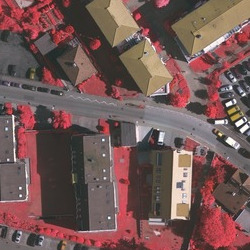
\includegraphics[width=\textwidth]{top}
    \caption{Image IRRV}
  \end{subfigure}
%   \begin{subfigure}[t]{0.19\textwidth}
%     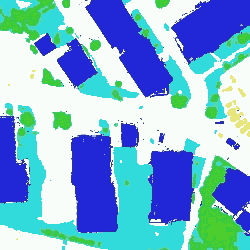
\includegraphics[width=\textwidth]{svl}
%     \caption{``SVL''\cite{gerke_use_2015}}
%   \end{subfigure}
    \begin{subfigure}[t]{0.19\textwidth}
    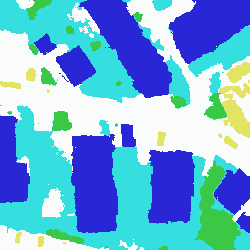
\includegraphics[width=\textwidth]{rf}
    \caption{RF + CRF\cite{quang_efficient_2015}}
  \end{subfigure}
    \begin{subfigure}[t]{0.19\textwidth}
    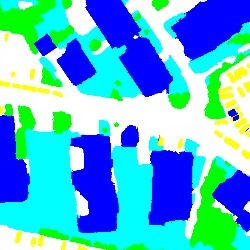
\includegraphics[width=\textwidth]{fcn}
    \caption{``DLR'' (FCN)\cite{marmanis_semantic_2016}}
  \end{subfigure}
    \begin{subfigure}[t]{0.19\textwidth}
    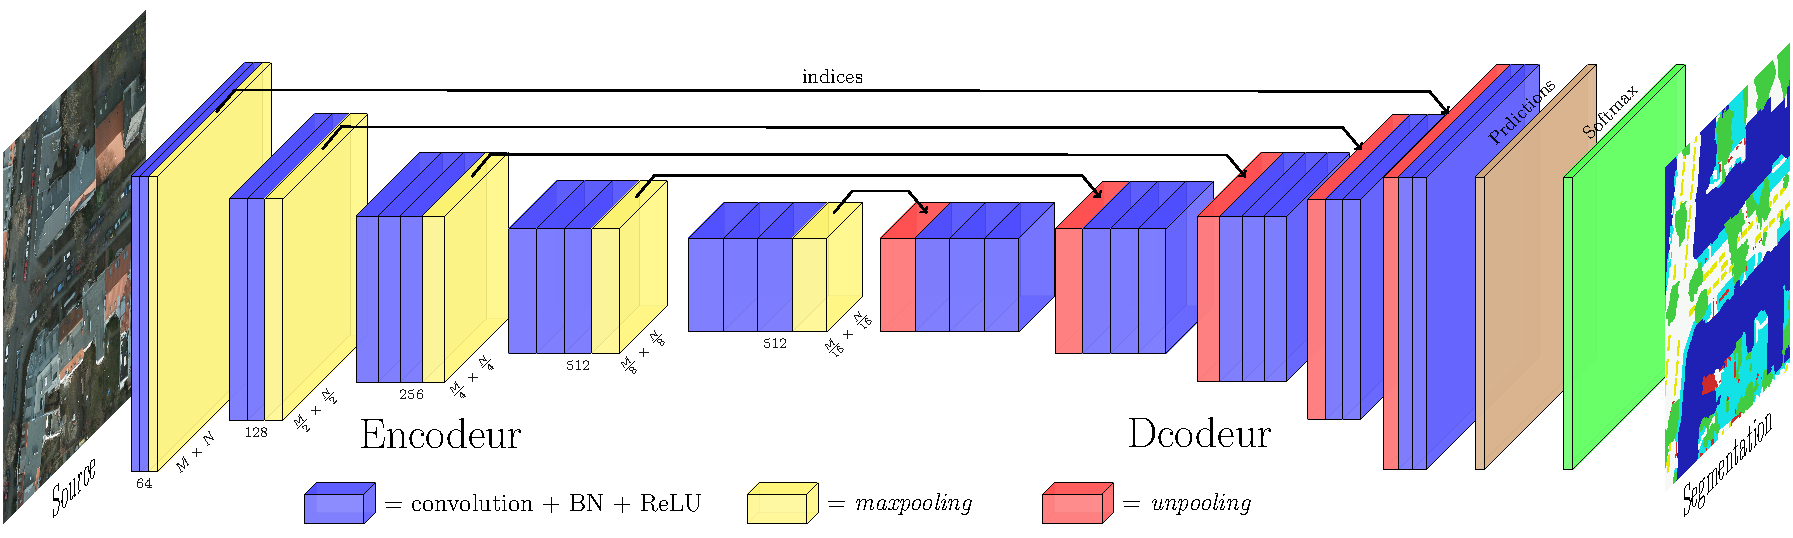
\includegraphics[width=\textwidth]{segnet}
    \caption{\textbf{SegNet++}}
  \end{subfigure}
  \caption{Comparaison des segmentations obtenues sur un extrait du jeu de test ISPRS Vaihingen.\\
  \isprslegende}
  \label{fig_segnet_qualitative}
\end{figure}

Comme démontré dans ~\cite{penatti_deep_2015}, les filtres convolutifs appris sur des images naturelles peuvent être efficacement transférées pour travailler sur des images aériennes. Toutefois, nous suggérons que de telles images présentent une régularité et une structure spatiale particulière liée au point de vue vertical utilisé. Ainsi, il peut exister un intérêt à laisser ces filtres pré-calculés être modifiés librement lors de l'optimisation du réseau. Pour évaluer cette hypothèse, nous comparons différents taux d'apprentissage pour l'encodeur ($lr_{e}$) et le décodeur ($lr_{d}$). Nous testons quatre stratégies~:
\begin{itemize}
  \item même variabilité~: $lr_{d} = lr_{e}$, ${lr_{e} / lr_{d}} = 1$,
  \item faible variabilité de l'encodeur: $lr_{d} = 2 \times lr_{e}$, ${lr_{e} / lr_{d}} = 0,5$,
  \item très faible variabilité de l'encodeur: $lr_{d} = 10 \times lr_{e}$, ${lr_{e} / lr_{d}} = 0,1$,
  \item absence de rétropropagation de l'erreur sur l'encodeur (aucune variabilité): $lr_{e} = 0$, ${lr_{e} / lr_{d}} = 0$.
\end{itemize}
Ces valeurs seront comparées avec l'initialisation aléatoire de tous les paramètres (encodeur et décodeur), correspondant à l'apprentissage d'un SegNet sans aucun pré-entraînement (et donc aucun transfert de connaissances).

Notre meilleur modèle améliore l'état-de-l'art sur le jeu de données ISPRS Vaihingen (cf. \cref{tab_leaderboard}) \footnote{Résultats détaillés : \url{http://www2.isprs.org/vaihingen-2d-semantic-labeling-contest.html}}. La \cref{fig_segnet_qualitative} illustre une comparaison qualitative entre différentes méthodes. Les métriques utilisées sont la qualité, définie comme le taux de bonne classification, et les scores F1 par classe~:
\begin{equation}
qualit\acute{e} = \frac{tp + tn}{tp + tn + fp + fn}
\end{equation}
\begin{equation}
F1_{i} = 2~\frac{pr\acute{e}cision_{i} \times rappel_{i}}{pr\acute{e}cision_{i} + rappel_{i}}
\end{equation}
\begin{equation}
rappel_i = \frac{tp_i}{C_i},~ pr\acute{e}cision_i = \frac{tp_i}{P_i}~,
\end{equation}

avec $tp, tn, fp, fn$ respectivement le nombre de vrais positifs, vrais négatifs, faux positifs et faux négatifs, $tp_i$ le nombre de vrais positifs de la classe $i$, $C_i$ le nombre de pixels appartenant à la classe $i$ et $P_i$ le nombre de pixels attribués à la classe $i$ par le modèle. Ces métriques sont calculées en ignorant un rayon de $3$ pixels autour des bordures afin de tenir compte d'éventuelles imprécisions dans la vérité terrain.

La meilleure méthode précédant notre soumission utilisait une combinaison de FCN et de caractéristiques expertes, tandis que la nôtre n'utilise que l'apprentissage statistique. La meilleure méthode précédente utilisant uniquement un FCN (``DLR\_1'') atteint 88,4\%, ce que nous améliorons de 1,4\%. Les précédentes méthodes utilisant les CNN atteignent 85,9\% (``ONE\_5''\cite{boulch_dag_2015}) et 86,1\% (``ADL\_1''\cite{paisitkriangkrai_effective_2015}). Notre méthode obtient des résultats supérieurs, sans recourir à des caractéristiques expertes ou à des post-traitement structurés comme les Champs Aléatoires Conditionnels ({\em Conditional Random Fields} - CRF). \cite{marmanis_classification_2017} obtient des résultats supérieurs en utilisant un ensemble de trois réseaux de neurones parallèles pour la fusion. Toutefois, cette méthode utilise un apprentissage multi-tâche incluant la prédiction de frontières comme régularisation et utilise un NDSM corrigé manuellement comme donnée additionnelle. Sans ce NDSM corrigé, le taux de bonne classification tombe à 89,4\%, un résultat inférieur à notre méthode.

\subsubsection{Recouvrement de la fenêtre glissante}

Autoriser un recouvrement dans la fenêtre glissante augmente le temps d'inférence mais accroît également la précision du modèle, comme détaillé dans le~\cref{tab_validation_results}. En effet, en divisant le pas par $2$, le nombre d'imagettes à traiter est multiplié par $4$. Cependant, moyenner plusieurs prédictions sur une même région permet de corriger des artefacts de classification, notamment le long des bords où le contexte spatial est manquant. L'expérience semble indiquer qu'un pas de $32$px (75\% de recouvrement) est suffisamment rapide pour la majorité des tâches et augmente significativement la précision (+1\%). Une tuile complète est ainsi traitée en 4 minutes sur une NVIDIA Tesla K20c avec un pas de $32$px et moins de 20 secondes avec un pas de $128$px. Le temps d'inférence est doublé dans le cas des deux SegNet parallèles.

\subsubsection{Transfert de connaissances}

Comme détaillé dans le~\cref{tab_initialization_results}, le modèle réalise sa meilleure performance lorsque le taux d'apprentissage de l'encodeur est relativement faible. Ceci renforce l'idée que des filtres convolutifs génériques donnent les meilleurs résultats lorsqu'il est possible de laisser l'optimisation les spécialiser sur une tâche particulière. Cependant, il est important de souligner qu'une variabilité trop grande induit un risque de surapprentissage. Ainsi, il est possible d'utiliser le taux d'apprentissage des paramètres pré-entraînés comme régularisation lors de l'optimisation. Ces résultats sont similaires aux conclusions de~\cite{nogueira_towards_2017} et aux observations générales de~\cite{yosinski_how_2014} concernant le transfert de connaissances.


\bibliographystyle{acm}
\bibliography{Chapitre2/Biblio}
